
\graphicspath{{part_4/figures}{part_4/figures/}}

\section{Introduction}


The computation of reachable sets for continuous-time dynamical
systems has been intensively studied during the last decades.
%While
%efficient methods to deal with linear dynamical systems have been
%defined \cite{LeGuernic2009,Bak2017}, the computation of reachable
%sets for non-linear systems is still a challenge.
Most of the methods
to compute the reachable set start from an \textit{initial value
  problem} for a system of \textit{ordinary differential equations} (ODE) defined
by
\begin{equation}
  \label{eq:ivp-ode}
  \dot{x}(t)=f(t,x(t))
  \quad\text{with}\quad x(0)\in X_0 \subset \mathbb{R}^n
  \quad\text{and}\quad t\in[0,t_{\text{end}}]\enspace.
\end{equation}
%Note that a {\em set} of initial values $X_0$ is considered in
%Equation~\eqref{eq:ivp-ode}.
As an analytical solution of
Equation~\eqref{eq:ivp-ode} is usually not computable, numerical
approaches have been considered.
%
A numerical method to solve Equation~\eqref{eq:ivp-ode}, when $X_0$ is
reduced to one value, produces a discretization of time, such that
$t_0 \leqslant \cdots \leqslant t_N = t_{\text{end}}$, and a sequence
of states $x_0$, \dots, $x_{N}$ based on an integration method
%$\Phi(f, x, t,h)$
which starts from an initial value $x_0$ at time
$t_0$ and a finite time horizon~$h$ (the step-size), produces an
approximation $x_{k+1}$ at time $t_{k+1} = t_k + h$, of the exact
solution $x(t_{k+1})$,
%\textit{i.e.}, $x(t_{n+1}; x_n) \approx \Phi(f, x_n,t_n,h)$
for all $k = 0,\dots,N-1$. The simplest numerical
method is Euler's method in which $t_{k+1} = t_k + h$ for some
step-size $h$ and $x_{k+1} = x_k + h f(t_k,x_k)$; so the derivative of
$x$ at time $t_k$, $f(t_k, x_k)$, is used as an approximation of the
derivative on the whole time interval.

%This method is very simple and
%fast, but requires small step-sizes $h$. More advanced methods, as for
%example the Runge-Kutta family, use a few intermediate computations to
%improve the approximation of the derivative.


The global error $error(t)$ at $t=t_0+kh$ is equal to
$\|x(t) -x_{k}\|$.  In case $n=1$, if the solution~$x$  has a bounded second derivative and $f$ is Lipschitz continuous in its second argument, then it
 satisfies:
\begin{equation}\label{eqn:error}
    error(t) \leq {\frac {hM}{2L}}(e^{L(t-t_{0})}-1)
  \end{equation}
%  \eqref{eqn:error}
%    $| GTE | \leq {\frac {hM}{2L}}(e^{L(t-t_{0})}-1)$

where $M$ is an upper bound on the second derivative of $x$ on the given interval and $L$
is the Lipschitz constant of $f$ \cite{atkinson2008introduction}.
\footnote{Such a bound has been used in hybridization methods:
$error(t)=\frac{E_D}{L}(e^{Lt}-1)$ \cite{asarin2007hybridization,chen2016decomposed},
where $E_D$ gives the maximum difference of the derivatives of the original and approximated systems.}\\

%%The classical result on Euler's method is an asymptotic result, saying that the error $\delta_n$ between the estimated result given by Euler's method after step~$n$ and the exact solution, converges to 0 as the number of steps $n=T/h$  tends to infinity (in O($n$)). This holds if the initial error $\delta_0$ is not ``too big''.

In \cite{SNR17}, we gave an upper bound on the global error $error(t)$,
which is more precise than (\ref{eqn:error}).
%under the form
%of a function $e$ (involving polynomials and exponentials) taking as arguments
%time $t$ and the initial error $\delta_{0}$ at time $t=0$.
%
This upper bound makes use of the notion of
{\em One-Sided Lipschitz (OSL)} constant. This notion has been used for the first
time by
\cite{donchev1998stability}
in order to treat ``stiff'' systems of differential equations for which the explicit Euler method is
numerically ``unstable'' (unless the step size is taken to be extremely small).
%have (in the case of linear equations) eigenvalues of very different modulus.
%The stability of systems governed by stiff equations is difficult to establish using only  Lipschitz constants.\footnote{The Euler method can also be numerically unstable, especially for stiff equations, meaning that the numerical solution grows very large for equations where the exact solution does not (Wikipedia).}
%
Unlike Lipschitz constants, OSL constants can be {\em negative},
which express a form of contractivity of the system dynamics.
Even if the OSL constant is positive, it is in practice much lower than
the Lipschitz constant \cite{dahlquist1976error}. The use of OSL thus allows us to obtain a much
more precise upper bound for the global error.
%$|x_n - x(t_n)|$.
%
We also explained in \cite{SNR17} how such a precise estimation of the
global error can be used to synthesize {\em safety controllers} for a special
form hybrid systems, called ``sampled switched systems''.\\

% In this paper,
% we explain how such an Euler-based method can be extended to synthesize safety controllers in a {\em distributed} manner. This allows us to control separately a component using only partial information on the other components. It also allows us to scale up the size of the global systems for which a control can be synthesized.\\



In this paper, we explain how such an Euler-based method can be extended to
synthesize safety controllers in a {\em distributed} manner. This allows us
to control separately a component using only partial information on the other
components. It also allows us to scale up the size of the global systems for
which a control can be synthesized. In order to perform such a distributed
synthesis, we will see the components of the global systems as being {\em interconnected}
(see, \textit{e.g.}, \cite{yang2015lyapunov}),
and use (a variant of) the notions of {\em incremental input-to-state stability ($\delta$-ISS)}
and {\em ISS Lyapunov functions}
\cite{jiang1996lyapunov}
instead of the notion of OSL used in the centralized framework.\\


The plan of the paper is as follows: In Section \ref{sec:background}, we recall the
results of \cite{SNR17} obtained in the centralized framework; in Section \ref{sec:distributed}
we extend these results to the framework of distributed systems;
we then apply the distributed synthesis method to a nontrivial example
(Section~\ref{sec:application}), and conclude in Section~\ref{sec:conc_part4}.


\section{Euler's method applied to control synthesis}\label{sec:background}
In this Section, we recall the results obtained in \cite{SNR17}.
We first give results concerning a system governed by a single ODE system
(Section \ref{ss:ODE}), then consider results for a switched system composed
of several ODEs (Section \ref{ss:switch}).
\subsection{ODE systems}\label{ss:ODE}
We make the following hypothesis:
%
$$(H0)\quad
%\mbox{ For all  $j\in U$,
\mbox{ $f$ is a locally Lipschitz continuous map}.$$

%As in \cite{girard2010approximately},
We make the assumption that the vector field $f$ is such that the
solutions of the differential equation  (\ref{eq:sys_part4}) are defined. %, e.g. by assuming that the support of the vector field $f$ is compact.
We will denote by $\phi(t; x^0)$ the
solution at time~$t$ of the system:

\begin{equation}
\begin{aligned}
  \dot  x(t) & =  f( x(t)), \\
   x(0) & =   x^0. \\
%  \sigma(t) & =  j \in U \ \text{for} \ t
%  \in \lbrack k\tau , (k+1)\tau ),\ \ k=0,1,\dots
\end{aligned}
 \label{eq:sampled-sys_part4}
\end{equation}
%
Consider a compact and convex set  $S\subset\mathbb{R}^n$,
called ``safety set''.
%
We denote by~$T$ a compact overapproximation of the image by $\phi$ of $S$ for $0\leq t\leq \tau$, %and $j\in U$,
\textit{i.e.},~$T$ is such that
$$ T\supseteq \{\phi(t;x^0) \ |\  0\leq t\leq\tau, x^0\in S\}.$$
%%%%
The existence of $T$ is guaranteed by assumption $(H0)$. We know furthermore
by~$(H0)$ that there exists a constant $L>0$ such that:
%\label{hyp:2}
%For all $j \in U$, there exists a constant $L>0$ such that
\begin{equation}
\|  f( y)- f( x) \| \leq L \, \| y- x\|\quad \forall  x, y\in S.
\label{eq:lipschitz_part4}
\end{equation}
Let us define $C$:
%We have:
\begin{equation}
%L\|f_{j}(x)\|\leq C_0
C = \sup_{x\in S}\  L\|f(x)\|.
\quad
%\text{for all} \quad j\in U.
\label{eq:L_part4}
\end{equation}
%
We make the additional hypothesis
that the mapping $f$ is {\em one-sided Lipschitz} (OSL)
\cite{donchev1998stability}.
%, which are often verified on systems modeling
%real world applications such as temperature regulation in a building (eg., \cite{meyer2014ecc}):
%we consider
%%%The Lipschitz condition is classically assumed in order to ensure the existence of a (unique) integral solution $\phi_\sigma$
%(see, e.g., \cite{liberzon2012switching}).
%This assumption of strong monotony is original in the context of switched systems, as far as we know.
Formally:
%
$$(H1)
%\label{hyp:1}
\quad \mbox{ There exists a constant $\lambda\in \mathbb{R}$ such that}$$
\[
\langle  f( y)- f( x),  y- x \rangle \leq \lambda\, \| y- x\|^2\quad
\forall  x, y\in T,
\]
where $\langle \cdot, \cdot\rangle$ denotes the scalar product of two vectors of $\mathbb{R}^n$.
%\end{definition}
%
%\footnote{Let  $\lambda_{min} = \min_{j \in U} \lambda$.}

\vspace{1em}

\begin{remark}
Constants $\lambda$, $L$ and $C$   can
be computed using (constrained) optimization algorithms.
%See
%Section \ref{sec:experiment} for details.
%be computed with (constrained) optimization algorithms.
%In practice, they are computed before the synthesis step.
%, using Octave functions.
\end{remark}



Given an  initial point $\tilde{x}^0\in S$, we define the following ``linear approximate solution''~$\tilde{\phi}(t;\tilde{x}^0)$ for $t$ on $[0,\tau]$ by:
\begin{equation}
\tilde{\phi}(t;\tilde{x}^0) = \tilde  x^0 + t f(\tilde  x^0).
\label{eq:grossier_part4}
\end{equation}
%for $\sigma(t)=j$.
%\newline
%\vspace{1em}
%Note that formula~\eqref{eq:grossier_part4} is nothing else but the explicit forward Euler scheme with ``time step'' $t$. It is thus a {consistent} approximation of order $1$ in $t$
%of the exact solution of~\eqref{eq:sys_part4}
%$ x_\sigma(t)$
%under the hypothesis $\tilde  x^0= x^0$.
% We further suppose that we have
% \[
% \tilde x(t)\in R\quad \forall t\geq 0.
% \]
% %

%We wish to synthesize a guaranteed control $\sigma$ for $\phi_{\sigma}$
%using the approximate functions $\tilde{\phi}_\pi$.%\eqref{eq:grossier_part4}.
We define the closed ball of center $x\in\mathbb{R}^n$ and radius $r>0$, denoted $B(x,r)$, as the set $\{x'\in\mathbb{R}^n \ |\ \|x'-x\| \leq r\}$.


Given a positive real $\delta$, we now define the expression $\delta(t)$
which, as we will see in Theorem \ref{th:1_part4}, represents (an upper bound on)
the error associated to $\tilde{\phi}(t; \tilde{x}^0)$
(\textit{i.e.}, $\|\tilde{\phi}(t; \tilde{x}^0)-\phi(t; x^0)\|$).

\begin{definition}\label{def:4_part4}
%In case  $(H1)$ is not satisfied because $\lambda=\min_{j\in U} \lambda <0$, %(and $\delta \not\geq\frac{C_0\tau}{\lambda}$),
%the conclusion of Theorem \ref{prop:bound} still holds if $B(\tilde{\phi}(t;\tilde{x}^0),\delta)$
%is replaced by $B(\tilde{\phi}(t;\tilde{x}^0),\delta'(t))$
%with
Let $\delta$ be a positive constant. Let us define, for all $0\leq t\leq \tau$,
$\delta(t)$ as follows:
\begin{itemize}
\item  if $\lambda <0$:
$$\delta(t)=\left(\delta^2 e^{\lambda t}+
 \frac{C^2}{\lambda^2}\left(t^2+\frac{2 t}{\lambda}+\frac{2}{\lambda^2}\left(1- e^{\lambda t} \right)\right)\right)^{\frac{1}{2}}$$
%

\item if $\lambda = 0:$
$$\delta(t)= \left( \delta^2 e^{t} + C^2 (- t^2 - 2t + 2 (e^t - 1)) \right)^\frac{1}{2}$$




%\item if $\lambda = 0:$
%$$\delta(t)= \frac{C t^2}{2} + \delta$$

\item if $\lambda > 0:$
$$\delta(t)=\left(\delta^2 e^{3\lambda t}+
\frac{C^2}{3\lambda^2}\left(-t^2-\frac{2t}{3\lambda}+\frac{2}{9\lambda^2}
\left(e^{3\lambda t}-1\right)\right)\right)^{\frac{1}{2}}$$
%
\end{itemize}
\end{definition}

Note that $\delta(t)=\delta$ for $t=0$.
The function $\delta(\cdot)$ depends implicitly on parameter: $\delta\in\mathbb{R}$. In Section \ref{ss:switch}, we will use the notation $\delta'(\cdot)$
where the parameter is denoted by $\delta'$.
%\footnote{In case $\lambda \geq 0$, the radius of the safety ball computed by our method increases exponentially with~$t$.}
%The proof is a simple adaptation of the above proof.


\begin{theorem}\label{th:1_part4}

Given
an ODE system satisfying (H0-H1), consider
a point $\tilde{x}^0$
and a positive real $\delta$.
We have,
for all $x^0\in B(\tilde{x}^0,\delta)$, $t\in [0,\tau]$:

%$$\phi(t;x^0)\in B(\tilde{x}^0-t f(\tilde{x}^0), \gamma)$$
$$\phi(t;x^0)\in B(\tilde{\phi}(t;\tilde{x}^0),\delta(t)).$$
\end{theorem}

\begin{figure}[t]
  \centering
%  \begin{tabular}{cc}
    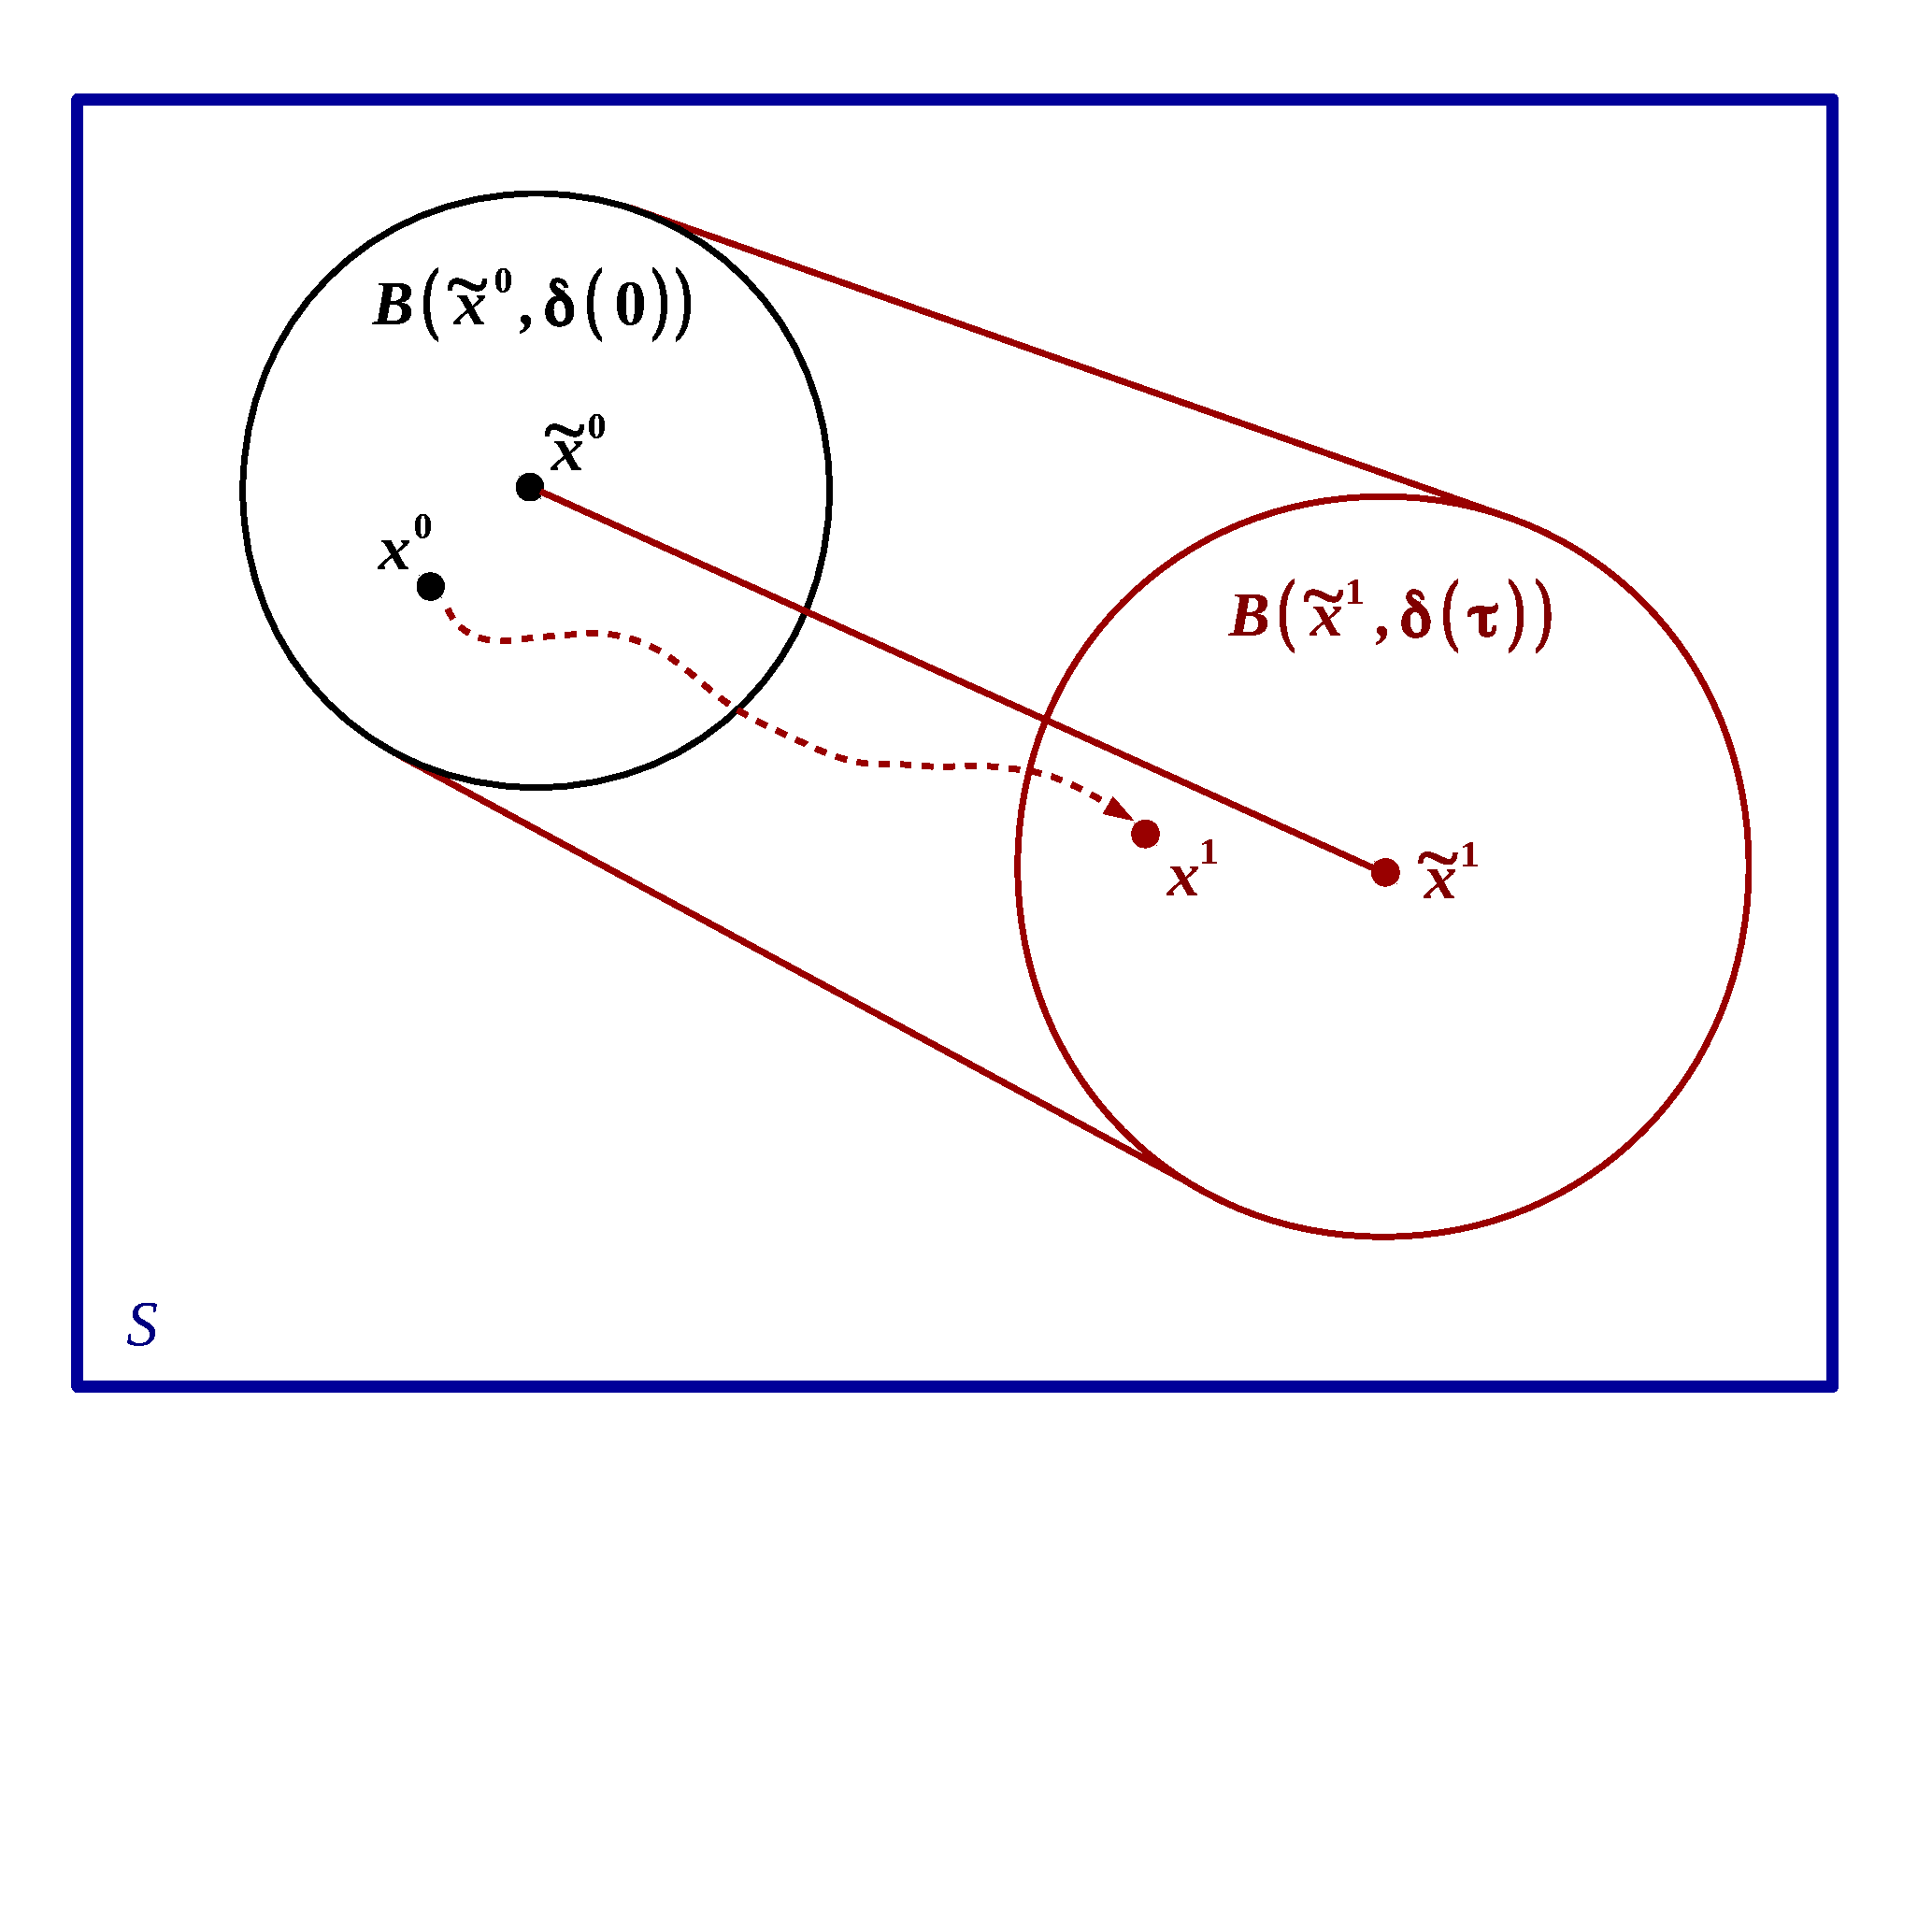
\includegraphics[width=0.49\textwidth,clip,trim = 0cm 9.5cm 0cm 0cm]{ball_image2.pdf}
    % &
    % 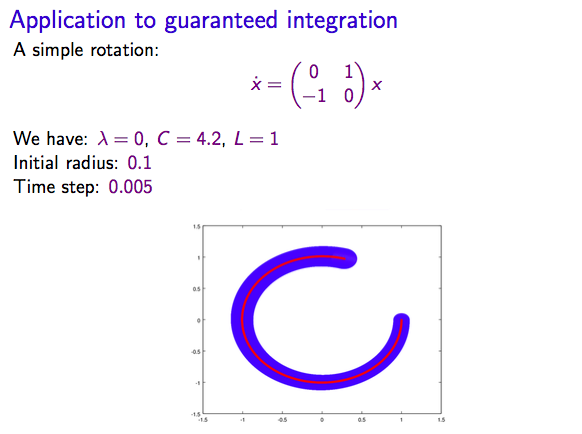
\includegraphics[width=0.49\textwidth]{rotation_Euler.png}
    % \\
    % (a) & (b)
%  \end{tabular}
  \caption{Illustration of Corollary \ref{cor:1_part4}, with $\tilde x_1 = \tilde{\phi}(\tau;\tilde{x}^0)$
    and $x_1 = {\phi}(\tau;{x}^0)$.}
  \label{fig:control_switch}
\end{figure}


\begin{corollary}\label{cor:1_part4}

Given an ODE system %\eqref{eq:sys_part4}
satisfying (H0-H1), consider
a point $\tilde{x}^0\in S$ and a real $\delta>0$ such that:
\begin{enumerate}
\item $B(\tilde{x}^0,\delta)\subseteq S$,
\item $B(\tilde{\phi}(\tau;\tilde{x}^0),\delta(\tau))\subseteq S$, and
\item $\frac{d^2(\delta(t))}{dt^2}>0$ for all $t\in [0,\tau]$.
\end{enumerate}
Then we have, for all $x^0\in B(\tilde{x}^0,\delta)$ and $t\in[0,\tau]$:\
%
%$\phi(t;x^0)\in B(\tilde{\phi}(t;\tilde{x}^0),\delta(t))\subseteq S$
$\phi(t;x^0)\in S$.


\end{corollary}
\subsection{Sampled switched systems}\label{ss:switch}
Let us consider the nonlinear switched system
\begin{equation}
 \dot  x(t) = f_{\sigma (t)}( x(t))
 \label{eq:sys_part4}
\end{equation}
defined for all $t \geq 0$, where $ x(t) \in \mathbb{R}^n$ is the state
of the system, $\sigma(\cdot) : \mathbb{R}^+ \longrightarrow U$ is the
switching rule. The finite set $U = \{ 1, \dots , N \}$ is the set of
switching {\em modes} of the system.  We focus on {\em sampled switched systems}:
given a sampling period $\tau >0$, switchings will occur at times
$\tau$, $2\tau$, \dots{} The switching rule~$\sigma(\cdot)$ is thus constant
on the time interval $\lbrack (k-1) \tau , k \tau )$ for $k \geq 1$.
For all $j\in U$, $f_j$ is a function from $\mathbb{R}^n$ to~$\mathbb{R}^n$.\\
% We call ``\emph{pattern}'' a finite sequence of modes $\pi =
% (i_1,i_2,\dots,i_k) \in U^k$.

We will denote by $\phi_\sigma(t; x^0)$ the
solution at time~$t$ of the system:

\begin{equation}
\begin{aligned}
  \dot  x(t) & =  f_{\sigma (t)}( x(t)), \\
   x(0) & =   x^0. \\
%  \sigma(t) & =  j \in U \ \text{for} \ t
%  \in \lbrack k\tau , (k+1)\tau ),\ \ k=0,1,\dots
\end{aligned}
 \label{eq:sampled-switch-sys}
\end{equation}
%


Often, we will consider $\phi_\sigma(t;x^0)$ on the interval $0\leq t<\tau$ for which $\sigma(t)$ is equal to a constant, say $j\in U$. In this case, we will abbreviate $\phi_\sigma(t;x^0)$ as $\phi_j(t;x^0)$. We will also consider $\phi_\sigma(t;x^0)$ on the interval $0\leq t<k\tau$
where $k$ is a positive integer, and
$\sigma(t)$ is equal to a constant, say $j_{k'}$,
on each interval
$[(k'-1)\tau,k'\tau)$ with $1\leq k'\leq k$; in this case,
we will abbreviate $\phi_\sigma(t;x^0)$ as $\phi_\pi(t;x^0)$,
where $\pi$ is a sequence of $k$ modes (or ``pattern'') of the form
$\pi=j_1\cdot j_2\cdot\dots\cdot j_k$.

We will assume that $\phi_\sigma$ is {\em continuous} at time $k\tau$ for all positive integer $k$.
This means that there is no ``reset'' at time $k'\tau$ ($1\leq k'\leq k$);
the value of
$\phi_\sigma(t,x^0)$ for $t\in[(k'-1)\tau,k\tau]$
corresponds to the solution of $\dot{x}(u)=f_{j_{k'}}(x(u))$  for $u\in [0,\tau]$
with initial value $\phi_\sigma((k'-1)\tau;x^0)$.\\

More generally, given an initial point $\tilde{x}^0\in S$ and  pattern $\pi$ of $U^k$,
we can define a ``(piecewise linear) approximate solution''
$\tilde{\phi}_\pi(t;\tilde{x}^0)$ of $\phi_\pi$ at time $t\in[0,k\tau]$ as follows:
\begin{itemize}
\item $\tilde{\phi}_\pi(t;\tilde{x}^0) = t f_j(\tilde{x}^0) + \tilde{x}^0$ if $\pi=j\in U$, $k=1$ and $t\in[0,\tau]$, and

\item $\tilde{\phi}_{\pi}(k\tau+t;\tilde{x}^0) = t f_j(\tilde{z}) + \tilde{z}$
with $\tilde{z}=\tilde{\phi}_{\pi'}((k-1)\tau;\tilde{x}^0)$, if $k\geq 2$,
$t\in[0,\tau]$,
$\pi=j\cdot \pi'$ for some $j\in U$ and $\pi'\in U^{k-1}$.
\end{itemize}

%{\bf NB: } We suppose that all the intermediate points $\tilde{z}$ belong to $S$ (\`a pr\'eciser)???.\\

We wish to synthesize a safety control $\sigma$ for $\phi_{\sigma}$
using the approximate functions $\tilde{\phi}_\pi$. %\eqref{eq:grossier_part4}.
%
Hypotheses (H0) and (H1), as defined in Section \ref{ss:ODE},
are naturally extended to every mode $j$ of $U$, as well as
definition of $T$, constants $L$, $C$ and~$\lambda$, definitions of
$\tilde{\phi}_j$ and $\delta$ (see \cite{SNR17}). From a notation point of view,
we will assign an index $j$ to symbols $\lambda, L, C,\dots$ in order to
relate them to the dynamics of mode $j$.\\

Consider a point~$\tilde{x}^0\in S$, a positive real  $\delta$ %\geq \frac{C_j\tau}{|\lambda_j|}$ for all $j\in U$,
and a pattern $\pi$ of length $k$.
Let $\pi(k')$ denote the $k'$-th element (mode) of~$\pi$ for $1\leq k'\leq k$.
Let us abbreviate
the $k'$-th approximate point
$\tilde{\phi}_{\pi}(k'\tau;\tilde{x}^{0})$
as~$\tilde{x}_\pi^{k'}$ for $k'=1,...,k$,
and let $\tilde{x}_\pi^{k'}=\tilde{x}^0$ for $k'=0$. It is easy to show that
$\tilde{x}_\pi^{k'}$ can be defined recursively for $k'=1,...,k$, by:
$\tilde{x}_\pi^{k'}=\tilde{x}_\pi^{k'-1}+\tau f_{j}(\tilde{x}_\pi^{k'-1})$
with $j=\pi(k')$.

Let us now
define the expression $\delta_\pi^{k'}$
%(an upper bound on) the error associated to $\tilde{x}_\pi^{k'}$,
%i.e. $\|\tilde{x}_\pi^{k'}- \phi_\pi(k'\tau;x^0)\|$.
%Using repeatedly Theorem \ref{th:1_part4},
%$\delta_{\pi}^{k'}$ can be defined recursively
as follows:
%\begin{itemize}
%\item
%(i.e., $\tilde{x}^{k'}=
%\tilde{x}^{k'-1} +\tau f_{\pi(k')}(\tilde{x}^{k'-1})$).
%\item
For $k'=0$: $\delta_{\pi}^{k'}=\delta$,
and for $1\leq k'\leq k$: $\delta^{k'}_{\pi}=\delta'_j(\tau)$
where $\delta'$ denotes $\delta^{k'-1}_{\pi}$, and $j$ denotes
$\pi(k')$.
%\end{itemize}
Likewise, for $0\leq t\leq k\tau$, let us
define the expression $\delta_{\pi}(t)$  as follows:
%(an upper bound on) the
%global error associated to $\tilde{\phi}_\pi(t;\tilde{x}^0)$
%(i.e.~$\|\tilde{\phi}_\pi(t;\tilde{x}^0)- \phi_\pi(t;x^0)\|$).
%Using Theorem \ref{th:1_part4},
%$\delta_{\pi}(t)$ can be defined itself as follows:
\begin{itemize}
\item for $t=0$:\ $\delta_\pi(t)=\delta$,
\item for $0<t\leq k\tau$:\
$\delta_{\pi}(t)=\delta'_{j}(t')$ with
$\delta'=\delta_\pi^{\ell-1}$, $j=\pi(\ell)$,
$t'=t-(\ell-1)\tau$ and
$\ell=\lceil \frac{t}{\tau}\rceil$.
\end{itemize}
Note that, for $0\leq k'\leq k$, we have:
$\delta_{\pi}(k'\tau)=\delta_\pi^{k'}$. We have
\begin{theorem}\label{th:safety}
  Given a sampled switched system satisfying (H0-H1), consider a
  point~$\tilde{x}^0\in S$, a positive real $\delta$ and a pattern
  $\pi$ of length $k$ such that, for all $1\leq k'\leq k$:
  \begin{enumerate}
  \item $B(\tilde{x}_\pi^{k'}, \delta_{\pi}^{k'}) \subseteq S$ and
  \item $\frac{d^2(\delta'_j(t))}{dt^2}>0$ for all $t\in [0,\tau]$,
    with $j=\pi(k')$ and $\delta'=\delta_\pi^{k'-1}$.
  \end{enumerate}
  Then we have, for all $x^0\in B(\tilde{x}^0,\delta)$ and $t\in
  [0,k\tau]$:\ \ $\phi_{\pi}(t;x^0)\in S$.
\label{prop:1bis_part4}
\end{theorem}

\begin{remark}
  In Theorem~\ref{prop:1bis_part4}, we have supposed that the step size $h$
  used in Euler's method was equal to the sampling period $\tau$ of
  the switching system.  Actually, in order to have better
  approximations, it is often convenient to take a {\em fraction} of
  $\tau$ as for $h$ (\textit{e.g.}, $h=\frac{\tau}{10}$).  Such a
  splitting is called ``sub-sampling'' in numerical methods.
\end{remark}

Consider now a compact set $R$, called ``recurrence set'', contained
in the safety set $S\subset\mathbb{R}^n$ ($R\subseteq S$). We are
interested in the synthesis of a control such that: starting from any
initial point $x\in R$, the controlled trajectory always returns to
$R$ within a bounded time while never leaving $S$.

\begin{corollary}
  \label{cor:cont}
  Given a switched system satisfying (H0-H1), consider a positive real
  $\delta$ and a finite set of points $\tilde{x}_1,\dots\tilde{x}_m$
  of $S$ such that all the balls $B(\tilde{x}_i,\delta)$ cover~$R$ and
  are included into~$S$ (\textit{i.e.}, $R\subseteq
  \bigcup_{i=1}^mB(\tilde{x}_i,\delta)\subseteq S$).

  Suppose furthermore that, for all $1\leq i\leq m$, there exists a
  pattern $\pi_i$ of length $k_i$ such that:
  \begin{enumerate}
    % \item $B(\tilde{\phi}_{\pi_i}(k'\tau;\tilde{x}_i),
    %   \delta_{\pi_i}(k'\tau)) \subseteq S$,
  \item $B((\tilde{x}_i)_{\pi_i}^{k'},\delta_{\pi_i}^{k'}) \subseteq
    S$, for all $k'=1,\dots,k_i-1$
%
\item
%$B(\tilde{\phi}_{\pi_i}(k_i\tau;\tilde{x}_i), \delta_{\pi_i}(k_i\tau)) \subseteq R.$
  $B((\tilde{x}_i)_{\pi_i}^{k_i}, \delta_{\pi_i}^{k_i}) \subseteq R.$
%
\item $\frac{d^2(\delta'_j(t))}{dt^2}>0$ with $j=\pi_i(k')$ and
  $\delta'=\delta_{\pi_i}^{k'-1}$, for all $k'\in\{1,...,k_i\}$ and
  $t\in [0,\tau]$.
%$\frac{d^2(\delta'_j(t)}{dt^2}>0$ for all $t\in [0,\tau]$, $j\in U$ and $\delta'\in [\delta]$.
\end{enumerate}
These properties induce a control $\sigma$\footnote{Given an initial
  point $x\in R$, the induced control $\sigma$ corresponds to a
  sequence of patterns $\pi_{i_1},\pi_{i_2},\dots$ defined as follows:
  Since $x\in R$, there exists a a point $\tilde{x}_{i_1}$ with $1\leq
  i_1\leq m$ such that $x\in B(\tilde{x}_{i_1},\delta)$; then using
  pattern $\pi_{i_1}$, one has: $\phi_{\pi_{i_1}}(k_{i_1}\tau;x)\in
  R$. Let $x'=\phi_{\pi_{i_1}}(k_{i_1}\tau;x)$; there exists a point
  $\tilde{x}_{i_2}$ with $1\leq i_2\leq m$ such that $x'\in
  B(\tilde{x}_{i_2},\delta)$, etc.}
%
which guarantees
%Let $k_{max}=\max_{i=1,\dots,m}\{k_i\}$.
\begin{itemize}
\item (safety): if $x\in R$, then $\phi_{\sigma}(t;x) \in S$ for all
  $t\geq 0$, and
\item (recurrence): if $x\in R$ then $\phi_{\sigma}(k\tau;x)\in R$ for
  some $k\in\{k_1,\dots,k_m\}$.
\end{itemize}
%
\label{prop:ter1_part4}
\end{corollary}

Corollary~\ref{prop:ter1_part4} gives the theoretical foundations of the
following method for synthesizing $\sigma$ ensuring recurrence in $R$
and safety in $S$:
\begin{itemize}
\item we (pre-)compute $\lambda_j, L_j, C_j$ for all $j\in U$;
\item we find $m$ points $\tilde{x}_1,\dots\tilde{x}_m$ of $S$ and
  $\delta>0$ such that $R\subseteq \bigcup_{i=1}^m
  B(\tilde{x}_i,\delta)\subseteq S$;
%for some $\delta>0$;%\geq \frac{C_j\tau}{\lambda}$;
\item we find $m$ patterns $\pi_i$ ($i=1,...,m$) such that conditions
  1-2-3 of Corollary~\ref{prop:ter1_part4} are satisfied.
\end{itemize}
%
A covering of $R$ with balls as stated in Corollary~\ref{prop:ter1_part4} is
illustrated in Figure~\ref{fig:post_part4}~(a).  The control synthesis
method based on~Corollary \ref{prop:ter1_part4} is illustrated in
Figure~\ref{fig:post_part4}~(b).
%(left)
%together with an illustration of method of \cite{NL_minimator} (right).




%  \begin{column}{0.48\textwidth}
 \begin{figure}[t]
 \centering
\begin{tabular}{cc}
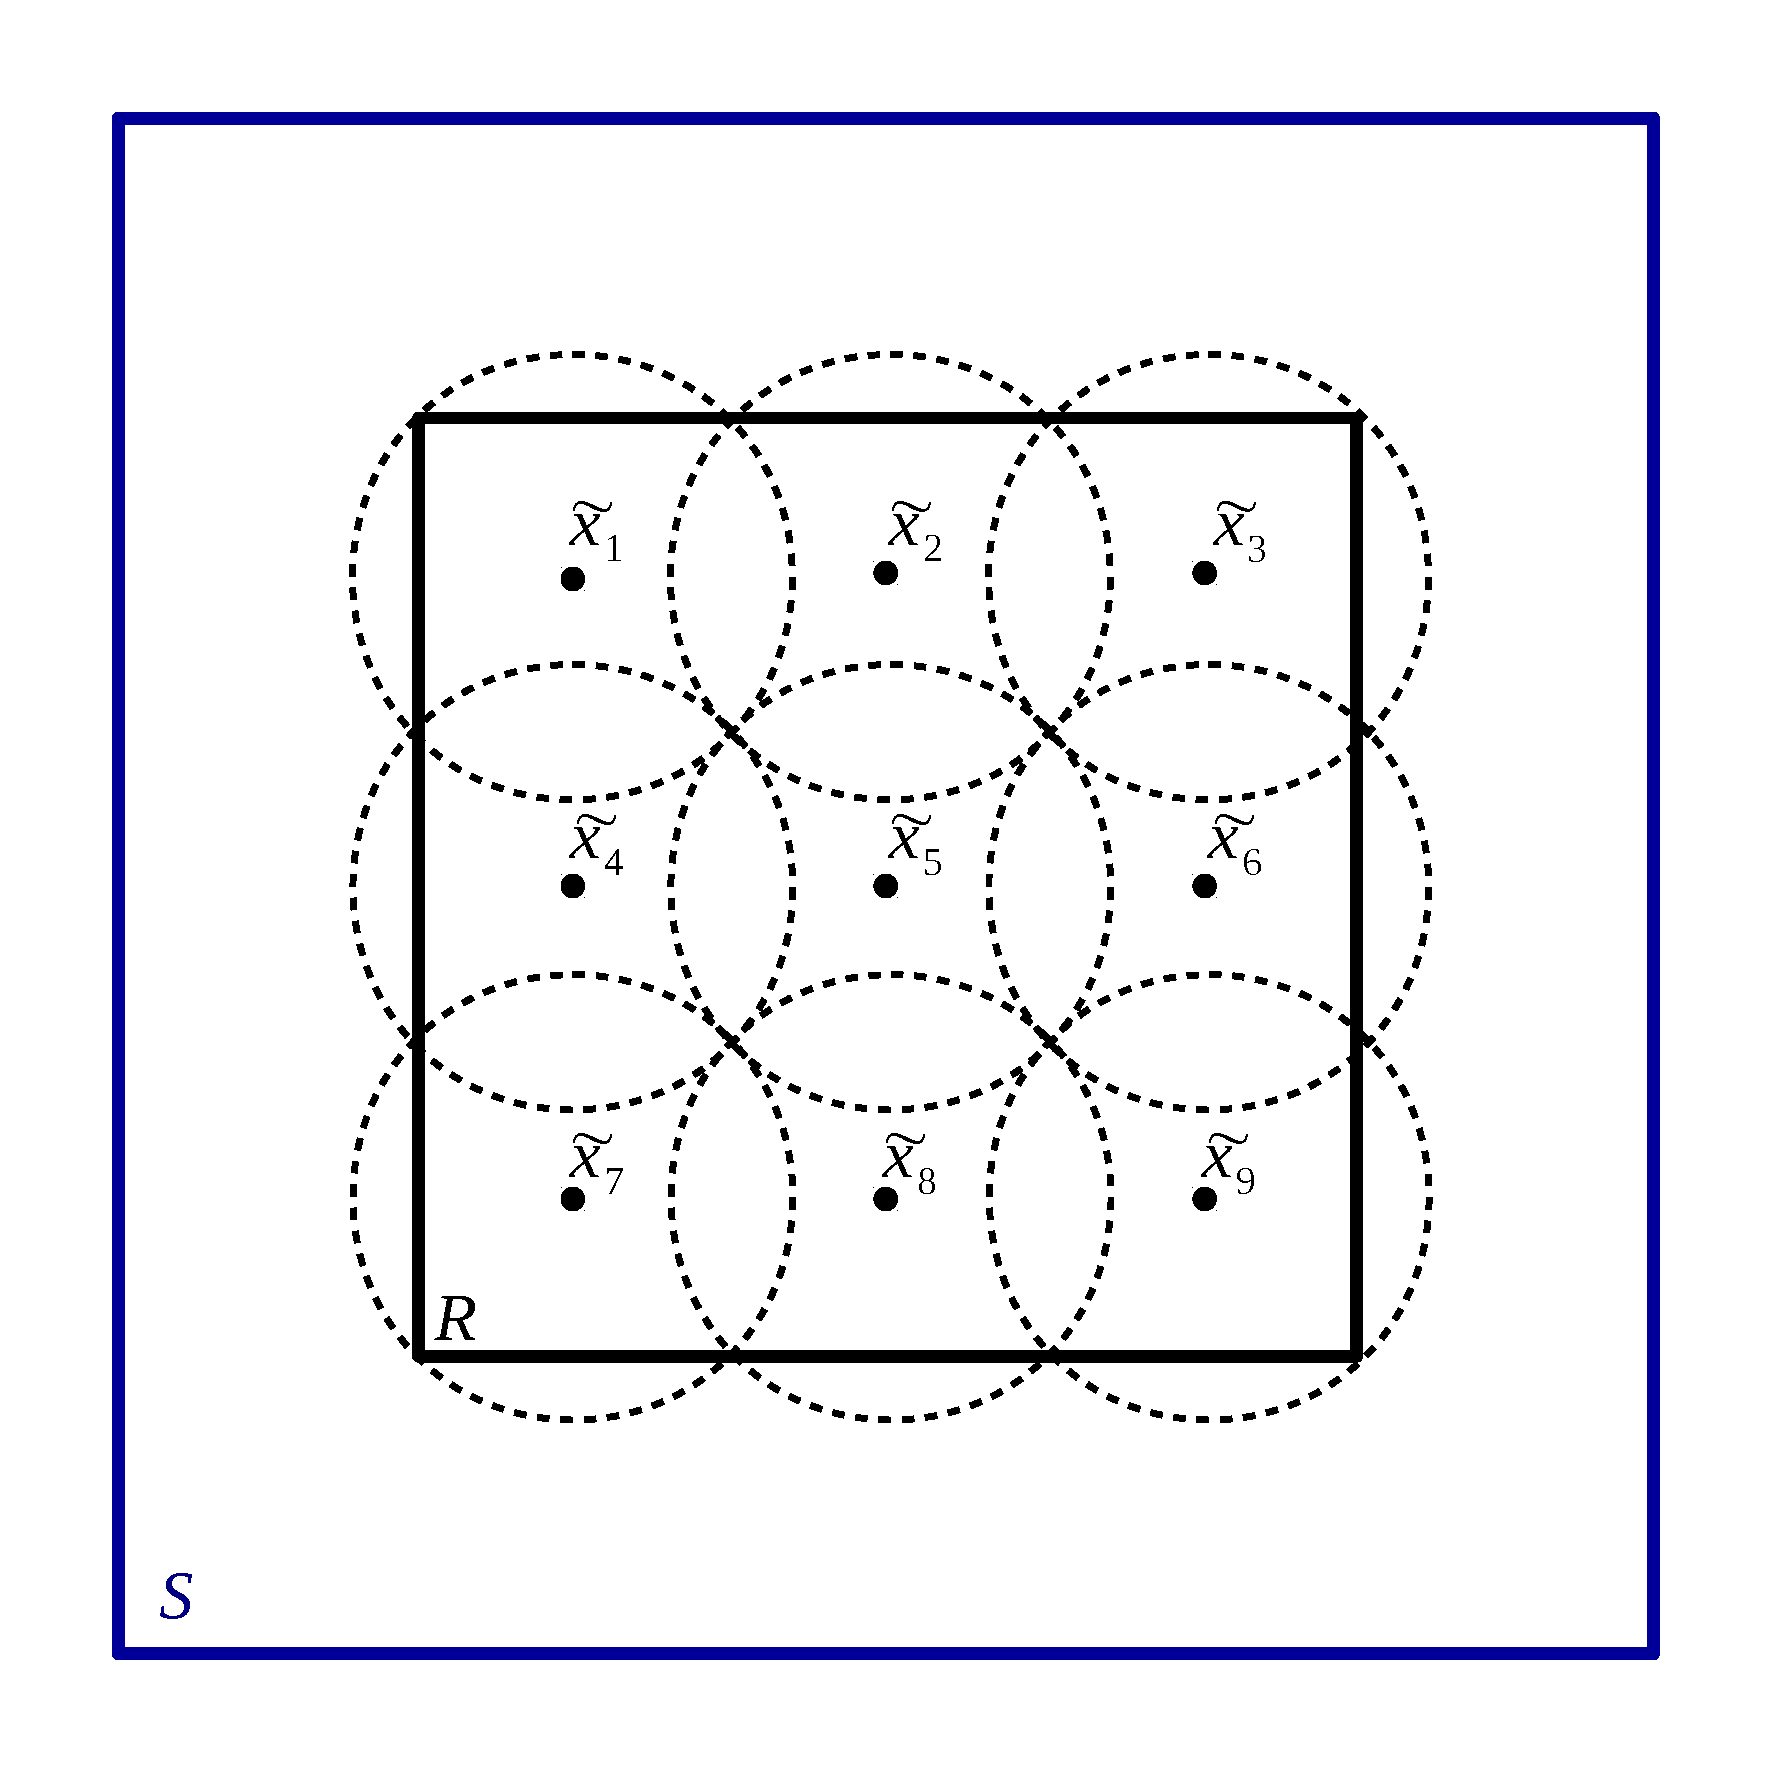
\includegraphics[width=0.42\textwidth,clip,trim=1cm 0cm 1cm 0cm]{tilingball2.pdf}
&
 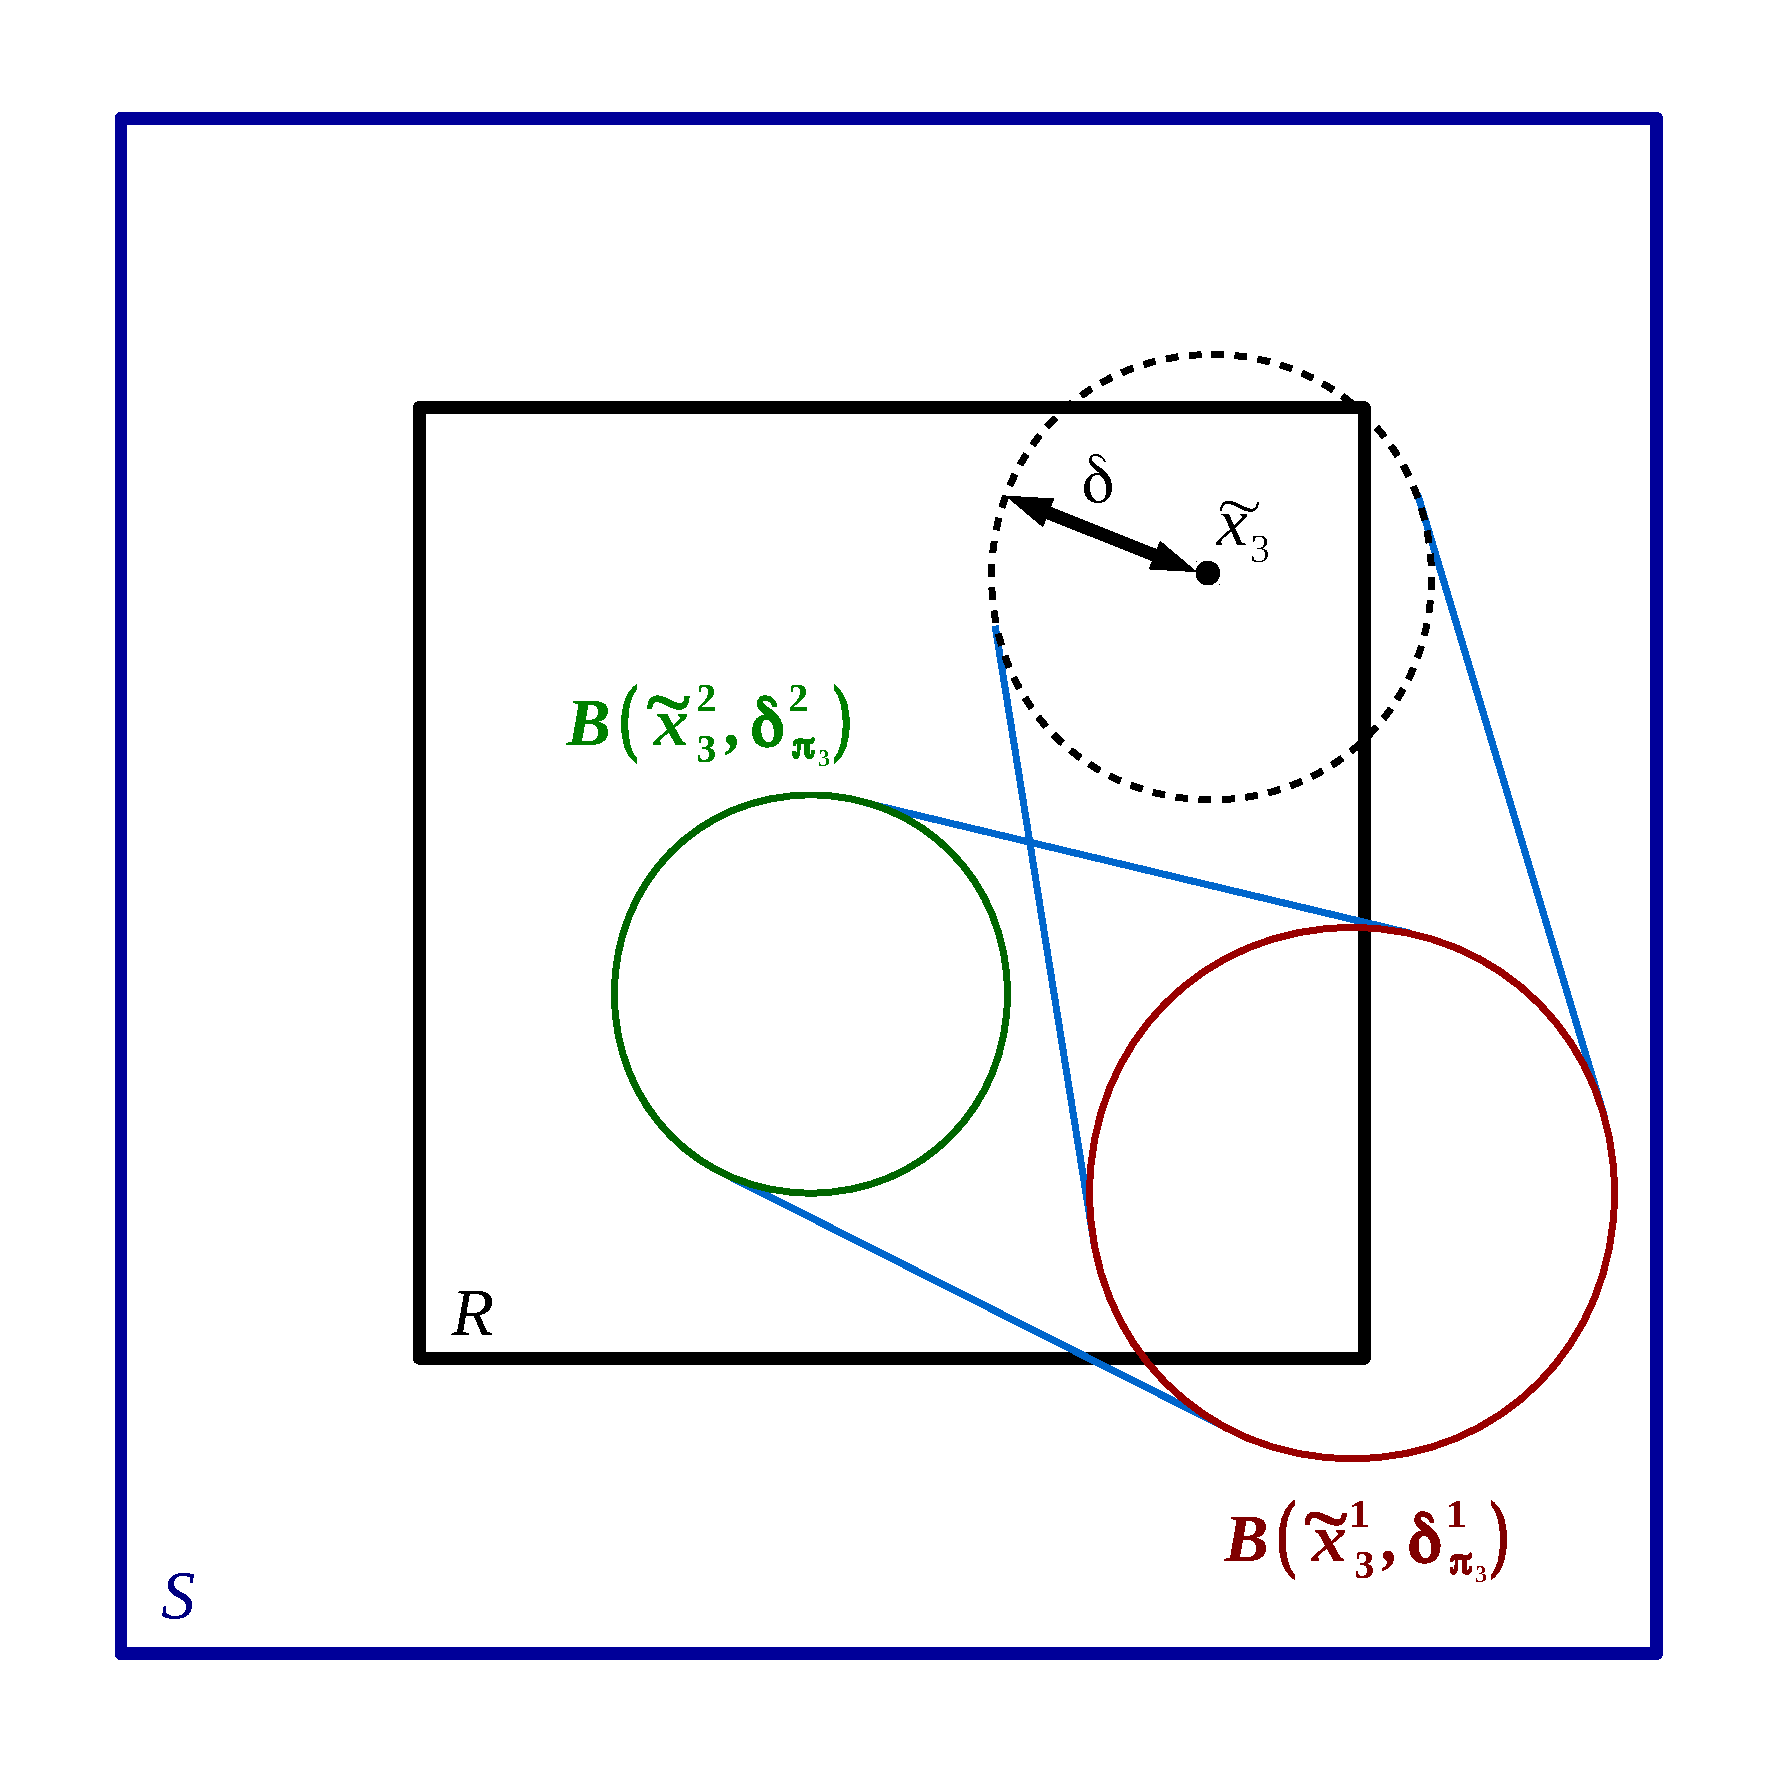
\includegraphics[width=0.42\textwidth,clip,trim=1cm 0cm 1cm 0cm]{tilingballimage.pdf}
 \\
 (a) & (b)
\end{tabular}
\caption{(a): A set of balls covering $R$ and contained in $S$. (b): Control of ball $B(\tilde x_3,\delta)$ with Euler-based method.}
\label{fig:post_part4}
\end{figure}







%\begin{remark}
%en fait vrai pour tout $0\leq t\leq k\tau$ (et pas seulement $0\leq t<k\tau$).
%\end{remark}

\section{Distributed synthesis}\label{sec:distributed}

The goal is to split the system into two (or more) sub-systems and
synthesize controllers for the sub-systems independently. The allows
to break the exponential complexity (curse of dimensionality) of the
method w.r.t. the dimension of the system, as well as the dimension of
the control input.

We consider the distributed control system
\begin{eqnarray}
 \dot x_1 = f_{\sigma_1}^1 (x_1,x_2)
  \label{eq:dist_sys1}\\
 \dot x_2 = f_{\sigma_2}^2 (x_1,x_2)
 \label{eq:dist_sys2}
\end{eqnarray}
where $x_1 \in \mathbb{R}^{n_1}$ and $x_2 \in \mathbb{R}^{n_2}$, with $n_1 + n_2 = n$.
Furthermore, $\sigma_1 \in U_1$ and $\sigma_2 \in U_2$ and $U = U_1 \times U_2$.
%

Note that the system (\ref{eq:dist_sys1}-\ref{eq:dist_sys2}) can be
seen as the {\em interconnection} of sub-system~(\ref{eq:dist_sys1})
where $x_2$ plays the role of an ``input'' given by
(\ref{eq:dist_sys2}), with sub-system~(\ref{eq:dist_sys2}) where $x_1$
is an ``input'' given by (\ref{eq:dist_sys1}).

%
Let $R = R_1 \times R_2$, $S = S_1 \times S_2$, $T = T_1 \times T_2$
and $x_1^m$ (resp. $x_2^m$) be the center of $R_1$ (resp. $R_2$).  We
denote by $L_{\sigma_1}^1$ the Lipschitz constant for sub-system~$1$
under mode $\sigma_1$:
$$ \| f_{\sigma_1}^1 (x_1,x_2) - f_{\sigma_1}^1 (y_1,y_2) \| \leq L_{\sigma_1}^1 \left\| \begin{pmatrix} x_1 \\ x_2 \end{pmatrix} - \begin{pmatrix} y_1 \\ y_2 \end{pmatrix} \right\|$$

We then introduce the constant:
$$ C_{\sigma_1}^1 = \sup_{x_1 \in S_1} L_{\sigma_1}^1 \| f_{\sigma_1}^1(x_1,x_2^m) \|$$
Similarly, we define the constants for sub-system~2:
$$ \| f_{\sigma_2}^2 (x_1,x_2) - f_{\sigma_2}^2 (y_1,y_2) \| \leq L_{\sigma_2}^2 \left\| \begin{pmatrix} x_1 \\ x_2 \end{pmatrix} - \begin{pmatrix} y_1 \\ y_2 \end{pmatrix} \right\|$$
and
$$ C_{\sigma_2}^2 = \sup_{x_2 \in S_2} L_{\sigma_2}^2 \| f_{\sigma_2}^2(x_1^m,x_2) \|$$

% We make the following assumption:
%
% $$(H2)
% %\label{hyp:1}
% \quad \mbox{For sub-system 1 and each mode $\sigma_1\in U_1$, there exist two real constants $\lambda^1_{\sigma_1}$ and $\gamma^1_{\sigma_1}$  such that}$$
% \[
% \langle f^1_{\sigma_1}(x_1,x_2) - f^1_{\sigma_1}(\tilde x_1,x_2^m), x_1 - \tilde x_1 \rangle \leq
% \lambda^1_{\sigma_1} \|x-x'\|^2 + \gamma^1_{\sigma_1} \|x-x'\| \|y-y'\|\, \quad
% \forall  x, x',  y, y'\in T
% \]
% and symmetrically for subsystem 2.\\


Let us now make additional assumptions on the coupled sub-systems,
closely related to the notion of (incremental) input-to-state
stability.

(H2) For every mode $\sigma_1 \in U_1$, there exists constants
$\lambda^1_{\sigma_1} \in \mathbb{R}$ and $\gamma^1_{\sigma_1} \in
\mathbb{R}_{>0}$ such that $\forall x,x' \in T_1^2$ and $\forall y,y'
\in T_2^2 $, the following expression holds
$$ \langle f_{\sigma_1}^1 (x,y) - f_{\sigma_1}^1 (x',y'), x - x' \rangle \leq \lambda^1_{\sigma_1} \| x - x' \|^2 + \gamma^1_{\sigma_1} \| x - x' \| \| y - y' \|. $$


(H3) For every mode $\sigma_2 \in U_2$, there exists constants
$\lambda^2_{\sigma_2} \in \mathbb{R}$ and $\gamma^2_{\sigma_2} \in
\mathbb{R}_{>0}$ such that $\forall x,x' \in T_1^2$ and $\forall y,y'
\in T_2^2 $, the following expression holds $$ \langle f_{\sigma_2}^2
(x,y) - f_{\sigma_2}^2 (x',y'), y - y' \rangle \leq
\lambda^2_{\sigma_2} \| y - y' \|^2 + \gamma^2_{\sigma_2} \| x - x' \|
\| y - y' \|. $$
%
% We consider the linear case and suppose that
% $$f_{\sigma_1}^1 (x_1,x_2) = A_{\sigma_1} x_1 + B_{\sigma_1} x_2 + u_{\sigma_1}$$
% and $$f_{\sigma_2}^2 (x_1,x_2) = A'_{\sigma_2} x_1 + B'_{\sigma_2}
% x_2 + u_{\sigma_2}$$

These assumptions express (a variant of) the fact that the function
$V(x,x')=\|x-x'\|^2$ is an {\em ISS-Lyapunov function} (see,
\textit{e.g.}, \cite{angeli2000lyapunov,hespanha2008lyapunov}).  Note
that all the constants defined above can be numerically computed using
constrained optimization algorithms.

Let us define the distributed Euler scheme:
\begin{eqnarray}
 \tilde x_1(\tau) = \tilde x_1(0) + \tau f_{\sigma_1}^1(\tilde x_1(0),x_2^m)
 \\
 \tilde x_2(\tau) = \tilde x_2(0) + \tau f_{\sigma_2}^2 ( x_1^m,\tilde x_2(0))
\end{eqnarray}

The exact trajectory is now denoted, for all $t \in [0,\tau]$, by
$\phi_{(j_1,j_2)}(t;x^0)$ for an initial condition $x^0
= \begin{pmatrix}x_1^0 & x_2^0\end{pmatrix}^T$, and when
sub-system~$1$ is in mode $j_1 \in U_1$, and sub-system~$2$ is in mode
$j_2 \in U_2$.

We define the approximate trajectory computed with the distributed
Euler scheme by $\tilde{\phi}_{j_ 1}^1(t;\tilde{x}_1^0) = \tilde x_1^0
+ t f_{\sigma_1}^1(\tilde x_1^0,x_2^m)$ for $t \in [0,\tau]$, when
sub-system~$1$ is in mode $j_1$ and with an initial condition $\tilde
x_1^0$. Similarly, for sub-system 2, $\tilde{\phi}_{j_
  2}^2(t;\tilde{x}_2^0) = \tilde x_2^0 + t f_{\sigma_2}^2(x_1^m,\tilde
x_2^0)$ when sub-system~$2$ is in mode $j_2$ and with an initial
condition~$\tilde x_2^0$.

We now give a distributed version of Theorem~\ref{th:1_part4}.
\begin{theorem}\label{th:1_part4bis}
  Given a distributed sampled switched system, suppose that
  sub-system~$1$ satisfies (H2), and consider a point $\tilde{x}_1^0$
  and a positive real $\delta$.
  % Let us denote by $\lambda_{j_1}$ the greatest eigenvalue of
  % $\frac{A_{j_1} + A_{j_1}^\top}{2}$ for all $j_1 \in U_1$.  Suppose
  % sub-system 1 verifies $$f_{\sigma_1}^1 (x_1,x_2) = A x_1 + B x_2 +
  % u_{\sigma_1}$$
  We have, for all $x_1^0\in B(\tilde{x}_1^0,\delta)$, $x_2^0 \in
  S_2$, $t\in [0,\tau]$, $j_1\in U_1$ and any $\sigma_2 \in U_2$:

  % $$\phi_j(t;x^0)\in B(\tilde{x}^0-t f_j(\tilde{x}^0), \gamma)$$
  $$\phi_{(j_1,\sigma_2)}(t;x^0)_{|1}\in B(\tilde{\phi}_{j_ 1}^1(t;\tilde{x}_1^0),\delta_{j_1}(t)).$$
  with $x^0 = \begin{pmatrix}x_1^0 & x_2^0\end{pmatrix}^T$ and
  \begin{itemize}
  \item if $\lambda^1_{j_1} <0$,
    \begin{multline}
      \delta_{j_1} (t) =
      % \frac{1}{\lambda^1_{j_1}^{3/2}}
      \left( \frac{(C_{j_1}^1)^2}{-(\lambda^1_{j_1})^4} \left( - (\lambda^1_{j_1})^2 t^2 - 2 \lambda^1_{j_1} t + 2 e^{\lambda^1_{j_1} t} - 2 \right) \right.   \\
      + \left. \frac{1}{(\lambda^1_{j_1})^2} \left( \frac{C_{j_1}^1 \gamma^1_{j_1} |S_2|}{-\lambda^1_{j_1}} \left( - \lambda^1_{j_1} t + e^{\lambda^1_{j_1} t} -1 \right) \right. \right.  \\ + \left. \left. \lambda^1_{j_1} \left( \frac{(\gamma^1_{j_1} )^2 (|S_2 |/2)^2}{-\lambda^1_{j_1}} ( e^{\lambda^1_{j_1} t } - 1) + \lambda^1_{j_1} \delta^2 e^{\lambda^1_{j_1} t}  \right) \right)  \right)^{1/2}
    \end{multline}
\item if $\lambda^1_{j_1} >0$,
  \begin{multline}
    \delta_{j_1} (t) = \frac{1}{(3\lambda^1_{j_1})^{3/2}} \left( \frac{C_1^2}{\lambda^1_{j_1}} \left( - 9(\lambda^1_{j_1})^2 t^2 - 6\lambda^1_{j_1} t + 2 e^{3\lambda^1_{j_1} t} - 2 \right) \right.   \\
    + \left. 3\lambda^1_{j_1} \left( \frac{C_1 \gamma^1_{j_1} |S_2|}{\lambda^1_{j_1}} \left( - 3\lambda^1_{j_1} t + e^{3\lambda^1_{j_1} t} -1 \right) \right. \right.  \\
    + \left. \left. 3\lambda^1_{j_1} \left( \frac{(\gamma^1_{j_1}) ^2 (|S_2 |/2)^2}{\lambda^1_{j_1}} ( e^{3\lambda^1_{j_1} t } - 1) + 3\lambda^1_{j_1} \delta^2 e^{3\lambda^1_{j_1} t}  \right) \right)  \right)^{1/2}
  \end{multline}
\item if $\lambda^1_{j_1} = 0$,
  \begin{multline}
    \delta_{j_1} (t) =
    % \frac{1}{\lambda_{j_1}^{3/2}}
    \left( {(C_{j_1}^1)^2} \left( -  t^2 - 2  t + 2 e^{ t} - 2 \right) \right.   \\
    + \left.  \left( {C_{j_1}^1 \gamma^1_{j_1} |S_2|} \left( -  t + e^{ t} -1 \right) \right. \right.  \\ + \left. \left.  \left({(\gamma^1_{j_1}) ^2 (|S_2 |/2)^2} ( e^{ t } - 1) +  \delta^2 e^{ t}  \right) \right)  \right)^{1/2}
  \end{multline}
\end{itemize}
\end{theorem}

% \begin{multline}
%  \delta_j (t) = \frac{1}{(3\vvvert A \vvvert)^{3/2}} \left( \frac{C_1^2}{\vvvert A \vvvert} \left( - 3\vvvert A \vvvert^2 t^2 - 6\vvvert A \vvvert t + 2 e^{3\vvvert A \vvvert t} - 2 \right) \right.   \\
%  + \left. 3\vvvert A \vvvert \left( \frac{C_1 \vvvert B \vvvert |S_2|}{\vvvert A \vvvert} \left( - 3\vvvert A \vvvert t + e^{3\vvvert A \vvvert t} -1 \right) \right. \right.  \\
%  + \left. \left. 3\vvvert A \vvvert \left( \frac{\vvvert B \vvvert ^2 |S_2 |^2}{\vvvert A \vvvert} ( e^{3\vvvert A \vvvert t } - 1) + 3\vvvert A \vvvert \delta^2 e^{3\vvvert A \vvvert t}  \right) \right)  \right)^{1/2}
% \end{multline}
A similar result can be established for sub-system 2, permitting to perform
a distributed control synthesis.

\begin{proof}

In order to simplify the reading, we omit the mode $j_1$ (which does not
intervene in the proof as long as $t \in [0,\tau]$) and write the proof
for $f_{j_1}^1 = f_1$, $L_{j_1}^1 = L_1$, $C_{j_1}^1 = C_1$,
$\lambda^1_{j_1} = \lambda_1$.  We have
\begin{align*}
  &\frac{1}{2} \frac{d (\| x_1 - \tilde x_1 \|^2)}{dt}
   = \langle
  f_1(x_1,x_2) - f_1(\tilde x_1(0),x_2^m),x_1 - \tilde x_1 \rangle
\\
  & = \langle f_1(x_1,x_2) - f_1(\tilde x_1,x_2^m) + f_1(\tilde
  x_1,x_2^m) - f_1(\tilde x_1(0),x_2^m),x_1 - \tilde x_1 \rangle
\\
& \leq \langle f_1(x_1,x_2) - f_1(\tilde x_1,x_2^m), x_1 - \tilde
  x_1 \rangle + \langle f_1(\tilde x_1,x_2^m) - f_1(\tilde
  x_1(0),x_2^m),x_1 - \tilde x_1 \rangle
  \\
& \leq \langle f_1(x_1,x_2) - f_1(\tilde x_1,x_2^m), x_1 - \tilde
  x_1 \rangle + \| f_1(\tilde x_1,x_2^m) - f_1(\tilde x_1(0),x_2^m) \|
  \|x_1 - \tilde x_1 \|
  \\
  & \leq \langle f_1(x_1,x_2) - f_1(\tilde x_1,x_2^m), x_1 - \tilde x_1 \rangle + L_1 \left\| \begin{pmatrix}
      \tilde x_1 \\ x_2^m \end{pmatrix} - \begin{pmatrix} \tilde x_1(0)
      \\ x_2^m \end{pmatrix} \right\| \|x_1 - \tilde x_1 \|
  \\
  & \leq \lambda_1  \| x_1 - \tilde x_1 \|^2 + \gamma_1  \| x_2 - x_2^m \| \| x_1 - \tilde x_1 \| + L_1 t \left\| f_1(\tilde x_1(0),x_2^m)
\right\| \|x_1 - \tilde x_1 \|
\\
& \leq \lambda_1 \| x_1 - \tilde x_1 \|^2 + \left( \gamma_1
  \frac{|S_2|}{2} + C_1 t \right) \|x_1 - \tilde x_1 \|
\end{align*}
where $|S_2|$ denotes the diameter of $S_2$.  Using the fact that
$\|x_1 - \tilde x_1 \| \leq \frac{1}{2} (\alpha \|x_1 - \tilde x_1
\|^2 + \frac{1}{\alpha}) $ for any $\alpha >0$, we can write three
formulas following the sign of $\lambda_1$.
\begin{itemize}
\item if $\lambda_1 <0$, we can choose $\alpha = \frac{-
    \lambda_1}{C_1 t + \gamma_1 |S_2|/2}$, and we get the differential
  inequality:
$$\frac{d (\| x_1 - \tilde x_1 \|^2)}{dt}  \leq \lambda_1 \|x_1 - \tilde x_1 \|^2  + \frac{C_1^2}{-\lambda_1} t^2 + \frac{C_1 \gamma_1 |S_2|}{-\lambda_1}t  + \frac{\gamma_1 ^2 (|S_2|/2)^2}{-\lambda_1}$$
\item if $\lambda_1 >0$, we can choose $\alpha = \frac{ \lambda_1
  }{C_1 t + \gamma_1 |S_2|/2}$, and we get the differential
  inequality:
$$\frac{d (\| x_1 - \tilde x_1 \|^2)}{dt}  \leq 3\lambda_1 \|x_1 - \tilde x_1 \|^2  + \frac{C_1^2}{\lambda_1} t^2 + \frac{C_1 \gamma_1 |S_2|}{\lambda_1}t  + \frac{\gamma_1 ^2 (|S_2|/2)^2}{\lambda_1}$$
\item if $\lambda_1 =0$, we can choose $\alpha = \frac{ 1 }{C_1 t +
    \gamma_1 |S_2|/2}$, and we get the differential inequality:
$$\frac{d (\| x_1 - \tilde x_1 \|^2)}{dt}  \leq \|x_1 - \tilde x_1 \|^2  + {C_1^2} t^2 + {C_1 \gamma_1 |S_2|}t  + {\gamma_1 ^2 (|S_2|/2)^2}$$
\end{itemize}

In every case, the differential inequalities can be integrated to
obtain the formulas of the theorem.

% \begin{multline}
%  \delta_j (t) = \frac{1}{(3\lambda_{max})^{3/2}} \left( \frac{C_1^2}{\lambda_{max}} \left( - 3\lambda_{max}^2 t^2 - 6\lambda_{max} t + 2 e^{3\lambda_{max} t} - 2 \right) \right.   \\
%  + \left. 3\lambda_{max} \left( \frac{C_1 \vvvert B \vvvert |R_2|}{\lambda_{max}} \left( - 3\lambda_{max} t + e^{3\lambda_{max} t} -1 \right) \right. \right.  \\
%  + \left. \left. 3\lambda_{max} \left( \frac{\vvvert B \vvvert ^2 |R_2 |^2}{\lambda_{max}} ( e^{3\lambda_{max} t } - 1) + 3\lambda_{max} \delta^2 e^{3\lambda_{max} t}  \right) \right)  \right)^{1/2}
% \end{multline}
\qed
 \end{proof}
%
%  We can now give a distributed version of Theorem \ref{th:safety}.
% \begin{theorem}
% Given a distributed sampled switched system satisfying of the form \eqref{eq:dist_sys1}-\eqref{eq:dist_sys2},
% %and an approximate  model \eqref{eq:sys_part42}.
% %
% consider a point~$\tilde{x}^0\in S$, a positive real  $\delta$ %\geq \frac{C_j\tau}{|\lambda_j|}$ for all $j\in U$,
% and a pattern $\pi_1$ of length $k_1$ such that, for all $1\leq k'\leq k_1$:
% \begin{enumerate}
% \item $B(\tilde{x}_\pi^{k'}, \delta_{\pi}^{k'}) \subseteq S$ and
% %
% \item $\frac{d^2(\delta'_j(t))}{dt^2}>0$ for all $t\in [0,\tau]$, with $j=\pi(k')$ and $\delta'=\delta_\pi^{k'-1}$.
% \end{enumerate}
% %
% Then we have, for all $x^0\in B(\tilde{x}^0,\delta)$ and $t\in [0,k\tau]$:\ \
% %$\phi_{\pi}(t;x^0)\in B(\tilde{\phi}_\pi(t;\tilde{x}^0), \delta_{\pi}(t)) \subseteq S$.
% $\phi_{\pi}(t;x^0)\in S$.
% %
% \label{prop:1bis_part4}
% \end{theorem}

It then follows a distributed version of Corollary~\ref{cor:cont}.
 \begin{corollary}\label{cor:cont_dist}
%Suppose that there is a tiling ${\cal R}={\cal R}_1\times{\cal R}_2$
%of $R$ of the
%form $\{r_{i_1}\times r_{i_2}\}_{(i_1,i_2)\in I_1\times I_2}$.
Given a positive real $\delta$, consider two sets of points
$\tilde x^1_{1},\dots,\tilde x^1_{m_1}$ and
$\tilde x^2_{1},\dots,\tilde x^2_{m_2}$ such that all the balls
$B(\tilde x^1_{i_1},\delta)$ and $B(\tilde x^2_{i_2},\delta)$, for $1 \leq i_1 \leq m_1$
and $1 \leq i_2 \leq m_2$,
cover $R_1$ and $R_2$.
Suppose that there exists patterns $\pi^1_{i_1}$ and $\pi^2_{i_2}$
of length $k_{i_1}$ and $k_{i_2}$
such that :

\begin{enumerate}
%\item $B(\tilde{\phi}_{\pi_i}(k'\tau;\tilde{x}_i), \delta_{\pi_i}(k'\tau)) \subseteq S$,
\item $B((\tilde{x}^1_{i_1})_{\pi^1_{i_1}}^{k'},\delta_{\pi^1_{i_1}}^{k'}) \subseteq S_1$,
for all $k'=1,\dots,k_{i_1}-1$
%
\item
%$B(\tilde{\phi}_{\pi_i}(k_i\tau;\tilde{x}_i), \delta_{\pi_i}(k_i\tau)) \subseteq R.$
$B((\tilde{x}^1_{i_1})_{\pi^1_{i_1}}^{k_{i_1}}, \delta_{\pi^1_{i_1}}^{k_{i_1}}) \subseteq R_1.$
%
{
\item $\frac{d^2(\delta'_{j_1}(t))}{dt^2}>0$
with $j_1=\pi_{i_1}^1(k')$ and $\delta'=\delta_{\pi_{i_1}^1}^{k'-1}$, for all
$k'\in\{1,...,k_{i_1}\}$ and $t\in [0,\tau]$.}
%$\frac{d^2(\delta'_j(t)}{dt^2}>0$ for all $t\in [0,\tau]$, $j\in U$ and $\delta'\in [\delta]$.
\end{enumerate}


\begin{enumerate}
%\item $B(\tilde{\phi}_{\pi_i}(k'\tau;\tilde{x}_i), \delta_{\pi_i}(k'\tau)) \subseteq S$,
\item $B((\tilde{x}^2_{i_2})_{\pi^2_{i_2}}^{k'},\delta_{\pi^2_{i_2}}^{k'}) \subseteq S_2$,
for all $k'=1,\dots,k_{i_2}-1$
%
\item
%$B(\tilde{\phi}_{\pi_i}(k_i\tau;\tilde{x}_i), \delta_{\pi_i}(k_i\tau)) \subseteq R.$
$B((\tilde{x}^2_{i_2})_{\pi^2_{i_2}}^{k_{i_2}}, \delta_{\pi^2_{i_2}}^{k_{i_2}}) \subseteq R_2.$
%
{
\item $\frac{d^2(\delta'_{j_2}(t))}{dt^2}>0$
with $j_2=\pi_{i_2}^2(k')$ and $\delta'=\delta_{\pi_{i_2}^2}^{k'-1}$, for all
$k'\in\{1,...,k_{i_2} \}$ and $t\in [0,\tau]$.}
%$\frac{d^2(\delta'_j(t)}{dt^2}>0$ for all $t\in [0,\tau]$, $j\in U$ and $\delta'\in [\delta]$.
\end{enumerate}
% $H1(\ell_1)$ and $H2(\ell_2)$ hold
% for some $\ell_1,\ell_2 \leq K$.
% Let $\ell=lcm(\ell_1,\ell_2)$ with $\ell=\alpha_1 \ell_1=\alpha_2 \ell_2$
% for some $\alpha_1,\alpha_2\in \mathbb{N}$.
%Consider the situation described in Proposition \ref{prop:basic}.
%Suppose furthermore that
%$| \pi_{1} | = |\pi_{j_1}|=\ell_1$ for all $i_1,j_1\in I_1$, and
%%
%$| \pi_{2} | = |\pi_{j_2}|=\ell_2$ for all $i_2,j_2\in I_2$.

The above properties induce a distributed control $\sigma = (\sigma_1,\sigma_2)$ guaranteeing
(non simultaneous) recurrence in $R$ and safety in $S$. \textit{I.e.}
\begin{itemize}
 \item if $x \in R$, then $\phi_\sigma (t;x) \in S$ for all $t\geq 0$

 \item if $x \in R$, then $\phi_\sigma ( k_1\tau;x)_{|1} \in R_1$ for some
 $k_1 \in \{ k_{i_1},\dots, k_{i_{m_1}} \}$, and symmetrically
 $\phi_\sigma ( k_2\tau;x)_{|2} \in R_2$ for some
 $k_2 \in \{ k_{i_2},\dots, k_{i_{m_2}} \}$
\end{itemize}


%
%
% %, starting from a point $x=(x_1,x_2)\in (R_1+a)\times (R_2+a)$,
% ${\cal R}_1$ induces a
% sequence of $\alpha_1$ macro-steps on $R_1+A$, and ${\cal R}_2$
% a sequence of $\alpha_2$ macro-steps on $R_2+A$, such that,
% when applied concurrently, we have
% for all $i_1\in I_1$ and $i_2\in I_2$:
% %macro-step\footnote{pas exactement ``one'',
% %mais $lcm(\ell_1,\ell_2)$ divis\'e par $\ell_1$ and $\ell_2$ respectivement} reachability uniform
% %distributed control
% %of horizon $K$
% \begin{multline}
% \Reach_f(\ell \tau,(r_{i_1}+A)\times (R_2+A),\pi)_{|1}\subseteq R_1 \ \wedge\\
% \Reach_f(\ell \tau,(R_1+A)\times (r_{i_2}+A),\pi)_{|2}\subseteq R_2,
% \end{multline}
% %$$ f(x,\pi)\in R,$$
% %, \mbox{ i.e., } f((x_1,x_2),(\pi_1^1\cdot \cdots \cdot\pi_1^{\alpha_1},
% %\pi_2^1\cdot \cdots \cdot\pi_2^{\alpha_2}))\in R_1\times R_2.$$
% for some $\pi=(\pi_1,\pi_2)\in \Pi^{\ell}$ where $\pi_1$ (resp. $\pi_2$)
% is of the form $\pi_1^1\cdots \pi_1^{\alpha_1}$
% (resp. $\pi_2^1\cdots \pi_2^{\alpha_2}$)
% with $\pi_1^i\in \Pi_1^{\ell_1}$  for all $1\leq i\leq \alpha_1$
% (resp. $\pi_2^i\in \Pi_2^{\ell_2}$  for all $1\leq i\leq \alpha_2$).
% %
% Hence:
% $$\Reach_f(\ell\tau,r_{i_1,i_2}+(A,A),\pi)\subseteq R.$$
% Besides, for all $0\leq t \leq \ell\tau$,
% we have:
% \begin{multline}
%   \Reach_f(t,(r_{i_1}+A)\times (R_2+A),\pi)_{|1}\subseteq R_1+A+\varepsilon\\
%   \wedge\ \Reach_f(t,(R_1+A)\times (r_{i_2}+A),\pi)_{|2}\subseteq R_2+A+\varepsilon.
% \end{multline}
% %
% %$$f(x,\pi')\in R+(a+\varepsilon,a+\varepsilon).$$
% Hence, for all $0\leq t \leq \ell\tau$:
% $$\Reach_f(t,r_{i_1,i_2}+(A,A),\pi)\subseteq R+(A+\varepsilon,A+\varepsilon).$$
\end{corollary}

 \section{Application}\label{sec:application}

We demonstrate the feasibility of our approach on a (linearized) building
ventilation application adapted from~\cite{meyer:tel-01232640}.
The~system is a four-room apartment subject to heat transfer between
the rooms, with the external environment and with the underfloor.
The dynamics of the system is given by the
following equation:
\begin{equation}
 \frac{d T_i}{dt} = \sum_{j \in \mathcal{N}^\text{*}\setminus \{i\}} a_{ij} (T_j -
 T_i)
%  + \delta_{s_i} b_i (T_{s_i}^4 - T_i ^4 )
%  \\
 + c_i
 \max\left(0,\frac{V_i - V_i^\text{*}}{\bar{ V_i} -
   V_i^{\text{*}}}\right)(T_u - T_i).
\end{equation}

The state of the system is given by the temperatures in the rooms
$T_i$, for $i \in \mathcal{N} = \{ 1 , \dots , 4 \}$.  Room $i$ is
subject to heat exchange with different entities stated by the indexes
$\mathcal{N}^\text{*} = \{1,2,3,4,u,o,c \}$.
%
The heat
transfer between the rooms is given by the coefficients $a_{ij}$ for
$i,j \in  \mathcal{N}^2$, and the different perturbations are the following:
\begin{itemize}
 \item The external environment: it has an effect on room $i$ with the
   coefficient $a_{io}$ and the outside temperature $T_o$, set to $30^\circ C$.
  \item The heat transfer through the ceiling: it has an effect on
    room $i$ with the coefficient $a_{ic}$ and the ceiling temperature
    $T_c$, set to $30^\circ C$.
  \item The heat transfer with the underfloor: it is given by the
    coefficient $a_{iu}$ and the underfloor temperature $T_u$, set to
    $17^\circ C$ ($T_u$ is constant, regulated by a PID controller).
%   \item The perturbation induced by the presence of humans: it is
%     given in room $i$ by the term $\delta_{s_i} b_i (T_{s_i}^4 - T_i
%     ^4 )$, the parameter $\delta_{s_i}$ is equal to $1$ when someone
%     is present in room $i$, $0$ otherwise, and $T_{s_i}$ is a given
%     identified parameter.
\end{itemize}

The control $V_i$, $i \in \mathcal{N}$, is applied through the term
$c_i \max(0,\frac{V_i - V_i^\text{*}}{\bar{ V_i} -
  V_i^{\text{*}}})(T_u - T_i)$.  A voltage $V_i$ is applied to force
ventilation from the underfloor to room $i$, and the command of an
underfloor fan is subject to a dry friction.  Because we work in a
switching control framework, $V_i$ can take only discrete values, which
removes the problem of dealing with a ``max'' function in interval
analysis. In the experiment, $V_1$ and $V_4$ can take the values $0$V
or $3.5$V, and $V_2$ and $V_3$ can take the values $0$V or $3$V. This
leads to a system of the form~\eqref{eq:sampled-switch-sys}
with $\sigma(t) \in U =\{
1, \dots, 16 \}$, the $16$ switching modes corresponding to the
different possible combinations of voltages $V_i$. The system can be decomposed in
sub-systems of the form \eqref{eq:dist_sys1}-\eqref{eq:dist_sys2}. The sampling
period is $\tau = 30$s.
The parameters $V_i^\text{*}$, $\bar V_i$, $a_{ij}$, $b_i$,
$c_i$ are given in~\cite{meyer:tel-01232640} and have been identified
with a proper identification procedure detailed
in~\cite{meyer2014ecc}.
% Note that here we have neglected the term
% $\sum_{j \in \mathcal{N}} \delta_{d_{ij}}c_{i,j} \ast h(T_j - T_i)$
% of~\cite{meyer:tel-01232640}, representing the perturbation induced by
% the open or closed state of the doors between the rooms.
% Taking a
% ``max'' function into account with interval analysis is actually still
% a difficult task. However, this term could have been taken into
% account with a proper regularization (smoothing).

The main difficulty of this example is the large number of modes in
the switching system, which induces a combinatorial issue.
%
%\fbox{parler de l'impl\'ementation, de la biblioth\`eque utilis\'ee...}
The centralized controller was obtained with $256$ balls in $48$
seconds, the distributed controller was obtained with $16 + 16$ balls
in less than a second. In both cases, patterns of length $2$ are used.
A sub-sampling of $h = \tau/20$ is required to obtain a controller
with the centralized approach. For the distributed approach,
no sub-sampling is required for the first sub-system, while the second
one requires a sub-sampling
of $h=\tau/10$.
% The
% perturbation due to human beings has been taken into account by
% setting the parameters $\delta_{s_i}$ equal to the whole interval
% $\lbrack 0,1 \rbrack$ for the decomposition, and the imposed
% perturbation for the simulation is given
% Figure~\ref{fig:NL_2_perturbation}.
% The temperatures $T_o$ and $T_c$
% have been set to the interval $\lbrack27,30\rbrack$ for the
% decomposition, and are set to $30^\circ C$ for the simulation.
Simulations of the centralized
and distributed controllers are given in Figure~\ref{fig:simu_4rooms}, where the control
objective is to stabilize the temperature in $\lbrack 20 , 22 \rbrack
^4$ while never going out of $\lbrack
19 , 23 \rbrack ^4$.

\begin{table}[t]
\label{table:4M_part4}
\caption{Numerical results for centralized four-room example.}
 \centering
%  {\tiny{
\begin{tabular}{|c|c|c|c|}
   \hline
   &\multicolumn{1}{c|}{Centralized}  \\
   \hline
   $R$ & \multicolumn{1}{c|}{$[20,22]^4$} \\
   $S$ & \multicolumn{1}{c|}{$[19,23]^4$} \\
\hline
$\tau$ & \multicolumn{1}{c|}{30} \\
\hline
Time subsampling & $\tau / 20$  \\
   \hline
 Complete control & Yes  \\
\hline
Error parameters &$\displaystyle\max_{j= 1, \dots,16} \lambda_j  =  -6.30\times 10^{-3}$     \\
&$\displaystyle\max_{j= 1, \dots,16} C_j  =  4.18\times 10^{-6}$ \\
\hline
Number of balls/tiles & 256 \\
Pattern length & 2 \\
\hline
CPU time &  48 seconds \\ \hline
  \end{tabular}
%   }}
 \end{table}




  \begin{table}[ht]
\label{table:4M_part42}
\caption{Numerical results for the distributed four-room example.}
 \centering
%  {\tiny{
\begin{tabular}{|c|c|c|}
\hline
& \multicolumn{1}{c|}{Sub-system 1} & \multicolumn{1}{c|}{Sub-system 2} \\
\hline
 $R$ & \multicolumn{2}{c|}{$[20,22]^2 \times [20,22]^2$} \\
   $S$ & \multicolumn{2}{c|}{$[19,23]^2\times[19,23]^2$} \\
\hline
$\tau$ & \multicolumn{2}{c|}{30} \\
\hline
Time subsampling & No & $\tau / 10$ \\
   \hline
 Complete control & Yes  & Yes \\
 Error parameters  & $\displaystyle\max_{j_1= 1, \dots,4} \lambda^1_{j_1} = -1.39 \times 10^{-3} $   & $\displaystyle\max_{j_2= 1, \dots,4} \lambda_{j_2}^2 = -1.42 \times 10^{-3} $   \\
 &  $\displaystyle \max_{j_1= 1, \dots,4} \gamma_{j_1}^1 = 1.79 \times 10^{-4} $        &   $\displaystyle\max_{j_2= 1, \dots,4} \gamma_{j_2}^2 = 2.47 \times 10^{-4} $      \\
& $\displaystyle\max_{j_1= 1, \dots,4} C^1_{j_1} =  4.15 \times 10^{-4} $   &  $\displaystyle\max_{j_2= 1, \dots,4} C^2_{j_2} =  5.75 \times 10^{-4} $ \\
Number of balls/tiles &  16 & 16 \\
Pattern length & 2  & 2\\
\hline
CPU time & $<1$ second &$<1$ second\\ \hline
\end{tabular}
 \end{table}

\begin{figure}[ht]
 \centering
 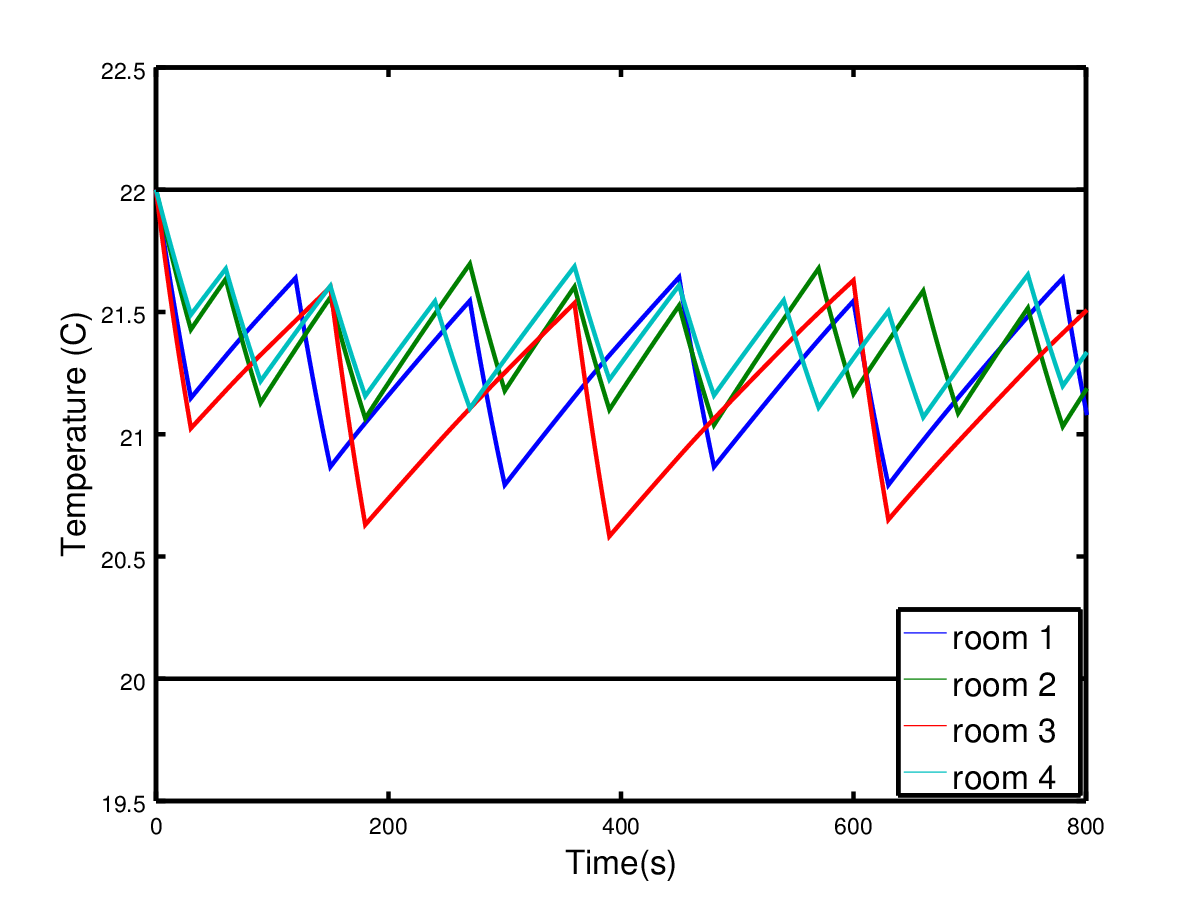
\includegraphics[scale=0.3]{simu_4rooms_central.png}%
% \caption{Simulation of the centralized controller from the initial condition $(22,22,22,22)$.}
%  \label{fig:NL_2}
%\end{figure}
%
%\begin{figure}[ht]
% \centering
%\hfill
 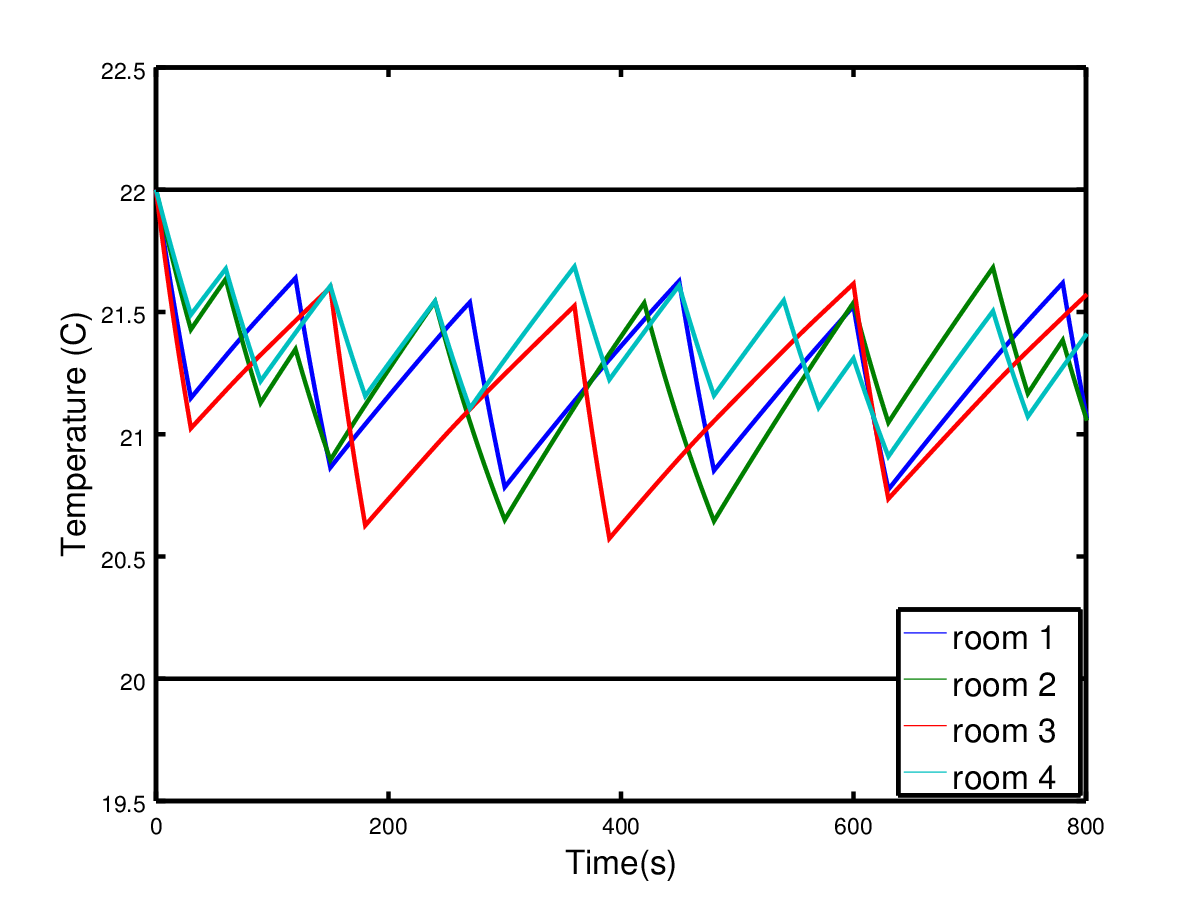
\includegraphics[scale=0.3]{simu_4rooms_compo.png}
 \caption{Simulation of the centralized (left) and distributed (right) controllers
 from the initial condition $(22,22,22,22)$.}
  \label{fig:simu_4rooms}
\end{figure}

 \section{Final remarks and future work}\label{sec:conc_part4}

 We have given a new distributed control synthesis method based on
 Euler's method.  The method makes use of the notions of
 $\delta$-ISS-stability and ISS Lyapunov functions.  From a certain
 point of view, this method is along the lines of
 \cite{dallal2015compositional} and \cite{kim2015compositional} which
 are inspired by small-gain theorems of control theory (see,
 \textit{e.g.}, \cite{jiang1994small}). In the future, we plan to
 apply our distributed Euler-based method to significant examples such
 as the 11-room example treated in
 \cite{larsen2015online,le2016distributed}.



%  \section{Appendix: Application to 2-room apartment}


%  We illustrate the approach with
% the example of a two rooms apartment, heated by two heaters located
% in each room (adapted from \cite{girard2012low}). In this example,
% the objective is to control the temperature of the two rooms. There is heat exchange between the
% two rooms and with the environment. The {\em continuous}
% dynamics of the system is given by the
% equation:
%  \[
%  \dot{\left( \begin{matrix}T_1 \\ T_2 \end{matrix} \right)}=\left(\begin{matrix} - \alpha_{21} - \alpha_{e1}-\alpha_f{ u_1} & \alpha_{21} \\
%  \alpha_{12} &-\alpha_{12}-\alpha_{e2} - \alpha_f u_2\end{matrix}
% \right)
% \left( \begin{matrix}T_1 \\ T_2 \end{matrix} \right) + \left( \begin{matrix}
%              \alpha_{e1} T_e + \alpha_f T_f { u_1} \\ \alpha_{e2}T_e + \alpha_fT_fu_2
%             \end{matrix}\right).
% \]
% Here $T_1$  and $T_2$ are the temperatures of the two rooms,
% and the state of the system corresponds to $T=(T_1,T_2)$.
% The control mode variable~$u_1$ (respectively~$u_2$)
%  can take the values $0$ or $1$
% depending on whether the heater in room~1 (respectively room~2)
%  is switched off or switched on (hence $U_1=U_2=\{0,1\}$).
% % Hence, here $n_1=n_2=1$, $N_1=N_2=2$ and $n=2,N=4$.
% %
% $T_e$~corresponds to the temperature of the
%  environment, and $T_f$ to the temperature of the heaters.
% %
%  The values of the different parameters are the following: $\alpha_{12} = 5 \times 10^{-2}$,
%  $\alpha_{21} = 5 \times 10^{-2}$, $\alpha_{e1} = 5 \times 10^{-3}$, $\alpha_{e2} = 5 \times 10^{-3}$,
%  $\alpha_{f} = 8.3 \times 10^{-3}$, $T_e = 10$ and $T_f = 35$.

%  {\color{red}

%  Pour le cas test, on peut obtenir un r\'esultat plus pr\'ecis que dans le cas g\'en\'eral
%  En reprenant la preuve:
%  $A = a$ est un scalaire (n\'egatif), on a }


% $$ \frac{1}{2} \frac{d (\| x_1 - \tilde x_1 \|^2)}{dt} = \langle f_1(x_1,x_2) - f_1(\tilde x_1(0),x_2^m),x_1 - \tilde x_1 \rangle $$

% $$ = \langle f_1(x_1,x_2) - f_1(\tilde x_1,x_2^m) + f_1(\tilde x_1,x_2^m) - f_1(\tilde x_1(0),x_2^m),x_1 - \tilde x_1 \rangle $$

% $$ \leq \langle f_1(x_1,x_2) - f_1(\tilde x_1,x_2^m), x_1 - \tilde x_1 \rangle + \langle f_1(\tilde x_1,x_2^m) - f_1(\tilde x_1(0),x_2^m),x_1 - \tilde x_1 \rangle $$

% $$ \leq \langle f_1(x_1,x_2) - f_1(\tilde x_1,x_2^m), x_1 - \tilde x_1 \rangle + \| f_1(\tilde x_1,x_2^m) - f_1(\tilde x_1(0),x_2^m) \| \|x_1 - \tilde x_1 \| $$

% $$ \leq \langle f_1(x_1,x_2) - f_1(\tilde x_1,x_2^m), x_1 - \tilde x_1 \rangle + L_1 \left\| \begin{pmatrix}
% \tilde x_1 \\ x_2^m \end{pmatrix} - \begin{pmatrix} \tilde x_1(0) \\ x_2^m \end{pmatrix} \right\| \|x_1 - \tilde x_1 \| $$

% $$ \leq \langle A(x_1 - \tilde x_1) + B( x_2 - x_2^m), x_1 - \tilde x_1 \rangle + L_1 t \left\| f_1(\tilde x_1(0),x_2^m)
% \right\| \|x_1 - \tilde x_1 \| $$

% $$ \leq  A  \| x_1 - \tilde x_1 \|^2 + \vvvert B \vvvert  \| x_2 - x_2^m \| \| x_1 - \tilde x_1 \| + L_1 t \left\| f_1(\tilde x_1(0),x_2^m)
% \right\| \|x_1 - \tilde x_1 \| $$

% $$ \leq  A  \| x_1 - \tilde x_1 \|^2 + \vvvert B \vvvert  \frac{|R_2|}{2} \| x_1 - \tilde x_1 \| + L_1 t \left\| f_1(\tilde x_1(0),x_2^m)
% \right\| \|x_1 - \tilde x_1 \| $$

% $$ \leq  A  \| x_1 - \tilde x_1 \|^2 + \left(\vvvert B \vvvert  \frac{|R_2|}{2}  + C_1 t \right) \|x_1 - \tilde x_1 \| $$

% Using the fact that $\|x_1 - \tilde x_1 \| \leq   \frac{1}{2} (\alpha \|x_1 - \tilde x_1 \|^2 + \frac{1}{\alpha}) $ for any $\alpha >0$,
% and choosing $\alpha = \frac{- A }{C_1 t + \vvvert B \vvvert |R_2|/2}$, we get the differential
% inequality:

% $$\frac{d (\| x_1 - \tilde x_1 \|^2)}{dt}  \leq A  \|x_1 - \tilde x_1 \|^2  + \frac{C_1^2}{-A} t^2 + \frac{C_1 \vvvert B \vvvert |R_2|/2}{-A}t  + \frac{\vvvert B \vvvert ^2 (|R_2|/2)^2}{-A}$$

% which can be integrated to obtain the formula:

% \begin{multline}
%  \delta_j (t) =
% %  \frac{1}{A^{3/2}}
%  \left( \frac{C_1^2}{-A^4} \left( - A^2 t^2 - 2 A t + 2 e^{A t} - 2 \right) \right.   \\
%  + \left. \frac{1}{A^2} \left( \frac{C_1 \vvvert B \vvvert |R_2|/2}{-A} \left( - A t + e^{A t} -1 \right) \right. \right.  \\
%  + \left. \left. A \left( \frac{\vvvert B \vvvert ^2 (|R_2 |/2)^2}{-A} ( e^{A t } - 1) + A \delta^2 e^{A t}  \right) \right)  \right)^{1/2}
% \end{multline}


% A distributed synthesis is performed with a sampling period $\tau =5$, in order to stabilize
% the temperature in the region $R = R_1 \times R_2 = [18,22] \times [18,22]$.
% The regions $R_1$ and $R_2$ are covered with $2$ balls each.
% Input sequences of length up to $2$ are used to stabilize the system.
% The computation time is under one second. Simulations
% of the induced controller is given in Figure \ref{fig:simu_compo} (b).

% By comparison, a centralized synthesis with the same region $R$ and sampling period $\tau$ requires
% a time sub-sampling ($h = \tau/10$) to prevent the error to grow and manage to stabilize the system.
% Input sequences of length up to $3$ are used, and the region $R$ is covered with $4$ balls.
% The computation time is comparable with the distributed case (under one second) for
% this low dimensional example. A simulation
% of the induced controller is given in Figure \ref{fig:simu_compo} (a).

% \begin{figure}
% \centering
% \begin{tabular}{cc}
%  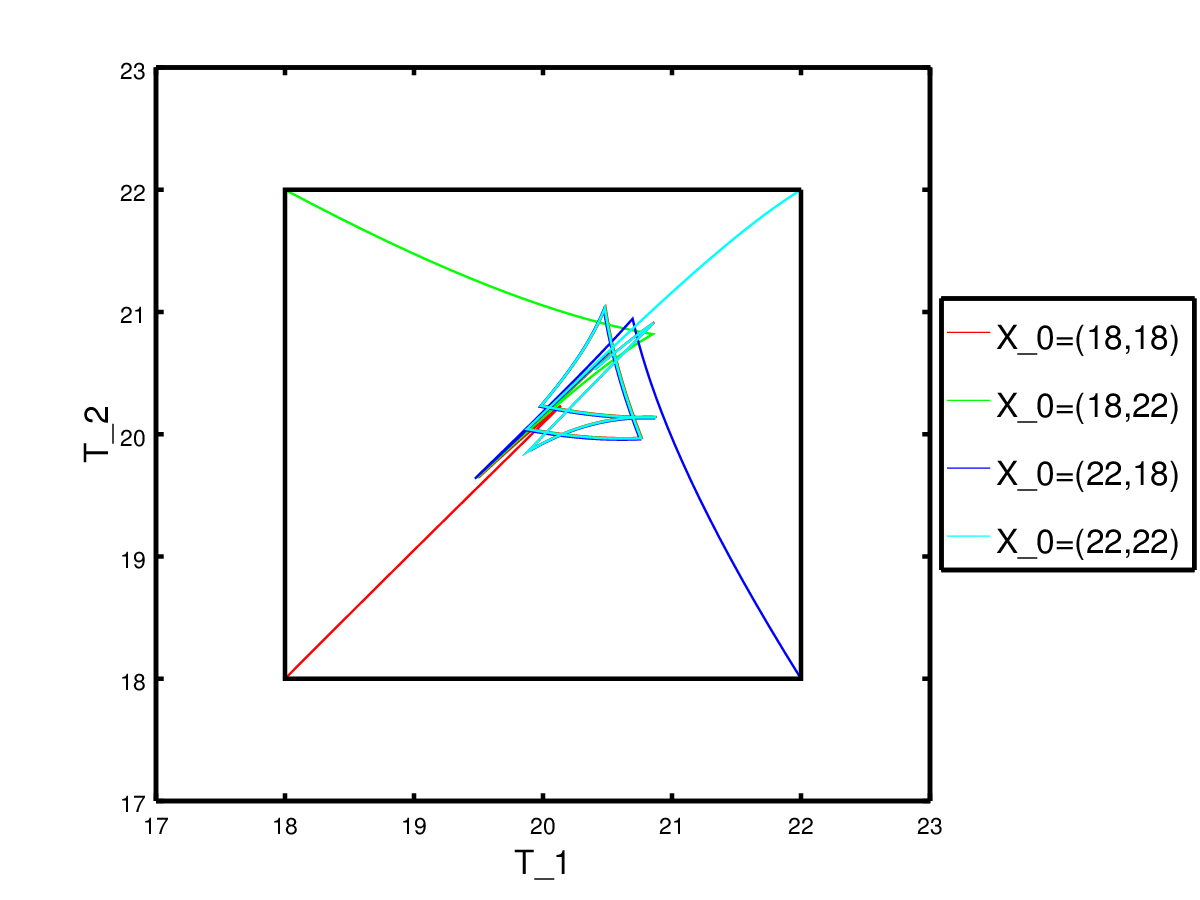
\includegraphics[width=0.49\textwidth]{simu_central.png}
%  &
%  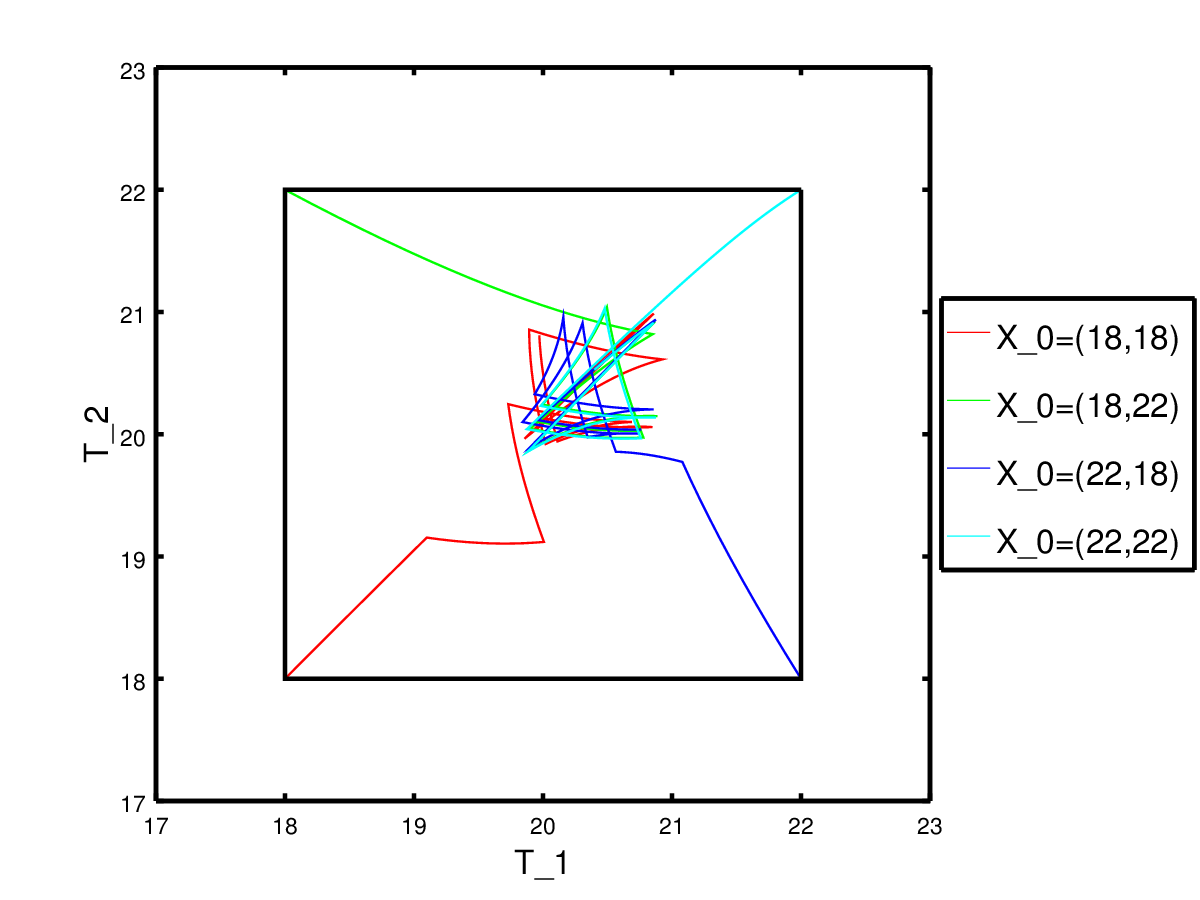
\includegraphics[width=0.49\textwidth]{simu_compo.png}
% \\
% (a) & (b)
% \end{tabular}

%  \caption{Simulation of the two-room example for four different initial conditions, with the centralized
%  synthesis algorithm (a), and the distributed algorithm (b).}
%  \label{fig:simu_compo}
% \end{figure}

% 
% 
% \todo[inline]{(Laurent) Remark: Donze et al. used sensitivity analysis to
%   compute the raidus of balls to cover the reachable sets of a
%   non-linear dynamical systems. It is different from the methods based
%   on Lipschitz constants. }
% 
% -----
% 
% \subsection{Comparison with methods of validated integration}
% \label{sec:one-sided-vs-validation-integration}
% 
% With Euler's method, we compute {\em points} (viewed as centers of balls of radius given by $e$). This is very different from the {\em polytope}-based approach used in classical methods of validated integration. An advantage of Euler's method is to avoid the difficulty of either computing successive polytopes with an increasing numbers of vertices, or enclosing the polytopes within convex hulls or parallelotopes, which may cause a wrapping effect. This is illustrated on Moore's rotation example in Figure~\ref{fig:rotation}.
% 
% \begin{figure}
% \centering
% \begin{tabular}{cc}
% % 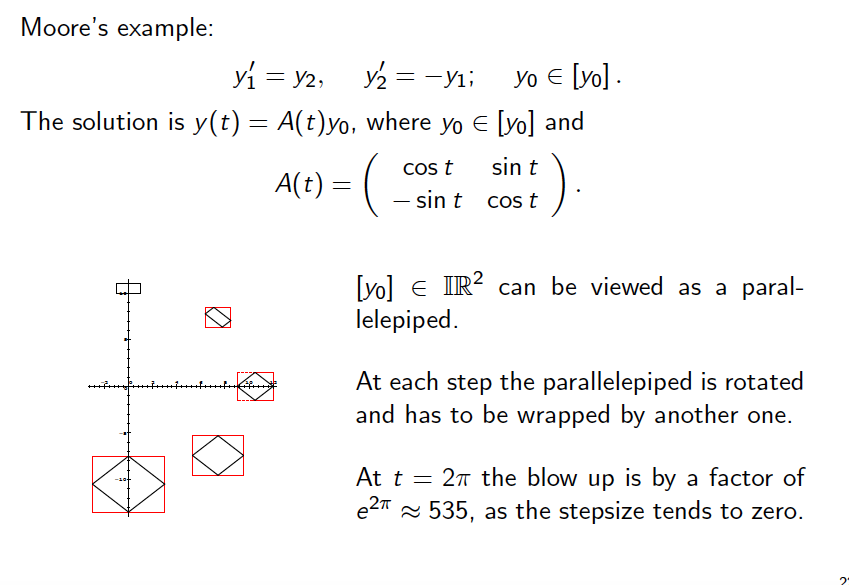
\includegraphics[width=0.49\textwidth]{Moore_rotation.png}
%   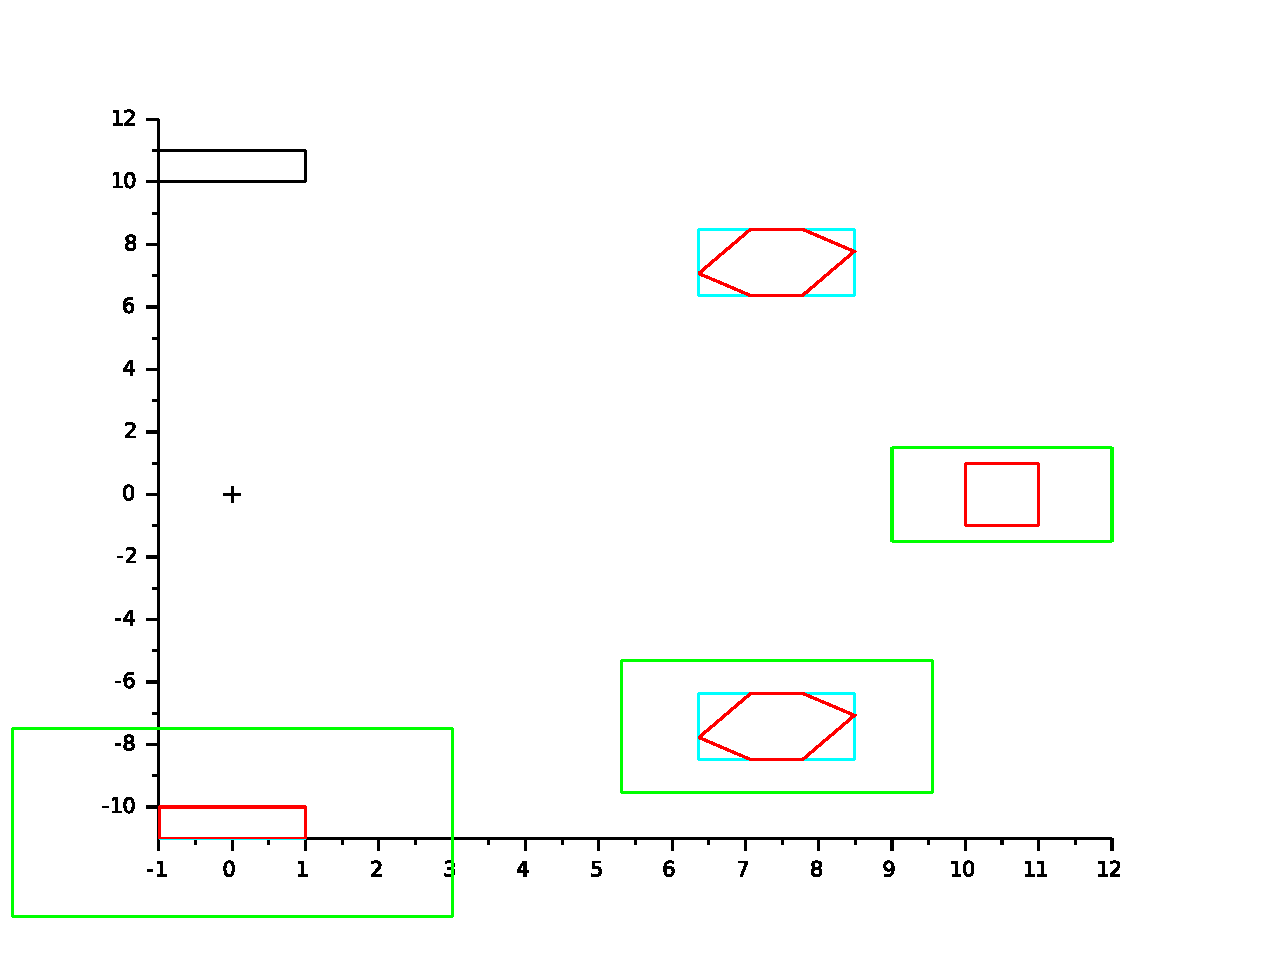
\includegraphics[width=0.49\textwidth]{figures/wrapping.pdf}
%  &
%  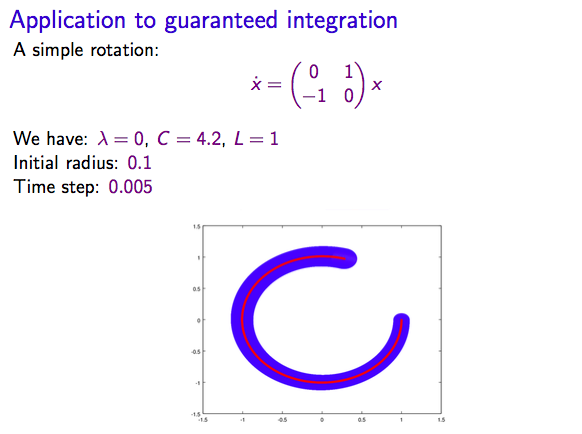
\includegraphics[width=0.49\textwidth]{rotation_Euler.png}
% \\
% (a) & (b)
% \end{tabular}
% 
%  \caption{Comparison of rotation Moore's example treated with
%  a basic interval method (a), Euler's method (b).}
%  \label{fig:rotation}
% \end{figure}
% 
% \todo[inline]{Changer cette figure avec celle de Moore 1966}
% 
% However all the methods presented in
% Section~\ref{sec:relat-work-reach} basically rely on initial Moore's
% paradigm which starts by enclosing all the trajectories between
% consecutive times $t_n$ and $t_{n+1}$ inside a parallepiped (see
% Figure \ref{fig:enclosure}). In contrast, our Euler-based method is a
% point-based approach which tries to bypass the wrapping effect in a
% radically alternative manner.
% 
% 
% 
% \todo[inline]{(Laurent) parler que one-sided Lipshictz est une méthode
%   ponctuelle et globale}
% 
% 
% ---------
% 
% A symbolic (or ``set-valued'') integration method consists in extend
% classical numerical integration methods by computing a set of states
% $X_j$, usually an over-approximation, at each time instants $t_j$ such
% that $X_j \supset \{ x(t_{j}; x_{j-1}) \mid \forall x_{j-1} \in
% X_{j-1} \}$.  To produce rigorous results, it is necessary to take
% into account approximation introduced by numerical method a.k.a.
% \textit{local truncation error} (LTE). LTE represents the distance
% between the true solution and the numerical solution, \textit{i.e.},
% $\|x(t_n; x_{n-1}) - x_n\|$. So in addition to function $\Phi$, the
% LTE function $\text{lte}_{\Phi}(f,\mathbf{x}_j,t_j,h)$ is added such
% that $X_j = \Phi(f, X_j,t_j,h) + \text{lte}_{\Phi}(f,X_j,t_j,h)$. In
% symbolic integration methods, the two main ingredients in methods to
% compute reachable sets are the geometric representation of sets and
% the propagation of sets with respect to the dynamical of the systems.
% 
% In applied mathematics, rigorous methods to study dynamical systems,
% mostly in order to produce results taking into account round-off errors
% due to floating-point arithmetic and numerical approximation due to
% the use of numerical methods to study dynamical systems. These
% approaches are known as \textit{validated numerical integration
%   methods} which took their root from the seminal work of R. Moore in
% using Taylor series methods
% \cite{Moore66,Lohner87,Nedialkov,LiSt07,Dzetkulic:2015fk,Makino2006346}.
% Recently methods based on other numerical schemes, mostly using
% Runge-Kutta methods, have been defined
% \cite{BM06,Gajda:2008fk,Rauh2009,BCD13,alexandreditsandretto:hal-01243044,alexandreditsandretto:hal-01243053}. All
% theses approaches can solve initial value problem for ordinary
% differential equations (ODEs) and some of them can deal with more
% complex dynamical systems such as differential-algebraic equations
% (DAEs) \cite{Rauh2009,alexandreditsandretto:hal-01243044}. All these
% approaches work in two steps: \textit{i)} Compute a bound
% $[\tilde{x}_j]$ of the solution over the time interval $[t_j,
% t_{j+1}]$ using interval Picard-Lindel\"of operator; \textit{ii)}
% compute a tightened value of the solution at time $t_{j+1}$ using
% either Taylor series or Runge-Kutta approaches. See
% Figure~\ref{fig:enclosure} as an illustration.
% 
% \begin{figure}
%   \centering
%   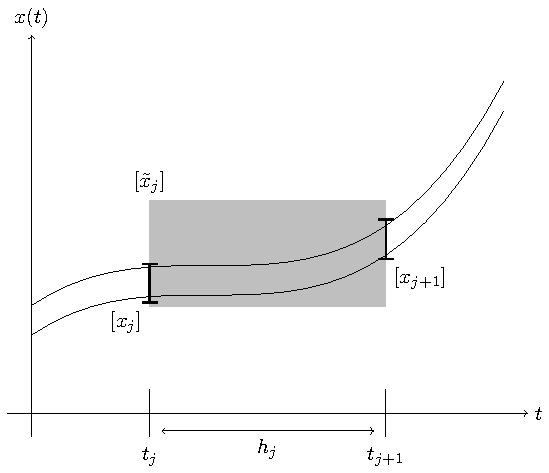
\includegraphics[scale=0.5]{figures/apriori.pdf}
%   \caption{Illustration of basic enclosure method for validated integration.}
% %   \label{fig:enclosure}
% \end{figure}
% 
% In validated numerical integration methods the most common
% representation of sets is based on boxes (Cartesian product of
% intervals) associated to special methods, for example the QR
% decomposition, see \cite{Lohner87}, to deal with pessimism introduce
% by the \textit{wrapping effect} (see
% Section~\ref{sec:one-sided-vs-validation-integration} for more
% details). Taylor Models \cite{Makino2006346} are an extension to
% interval arithmetic to deal with the pessimism of boxes.  The use of
% ellipsoids have also been considered in \cite{Neumaier1993}. Some
% recent work \cite{alexandreditsandretto:hal-01243053} based on
% Runge-Kutta methods uses zonotopes \cite{Kuhn:1998:RCO:287056.287083}
% to counter-act the wrapping effect. Note that theses approaches have
% been used to analyze or verify hybrid systems such as in
% \cite{DBLP:conf/hybrid/HenzingerHMW00,CAS12,Eggers:2012fk}. Note also
% that for special non-linear systems described by polynomials
% \cite{Dang:2012:RAP} methods based on set representation using
% Bernstein polynomials have been defined. Despite various approaches to
% represent sets of states, wrapping effect is still a challenge to
% address to produce sharp result of the reachable set.
% 
% % Since Moore 1966, the polytope-based method has been refined in a
% % considerable number of ways in order to fight the wrapping effect
% % (using zonotopes, affine arithmetic, interval ellipsoid arithmetic,
% % QR algorithm, Taylor models, etc.) [Loehner][A New Perspective on
% % the Wrapping Effect in Interval Methods for Initial Value Problems
% % for Ordinary Differential Equations, Nedialko S. Nedialkov, Kenneth
% % R. Jackson, 2001][The wrapping effect, ellipsoid arithmetic,
% % stability and confidence regions, Arnold Neumaier,
% % [R. Lohner. Enclosing the solutions of ordinary initial- and
% % boundary-value problems. In Computer arithmetic (E. Kaucher,
% % U. Kulisch, and Ch. Ullrich, eds.), pp. 255–286. Teubner, Stuttgart
% % (1987)][SUPPRESSION OF THE WRAPPING EFFECT BY TAYLOR MODEL- BASED
% % VALIDATED INTEGRATORS, KYOKO MAKINO AND MARTIN BERZ].
% 
% An exception of the two steps process of validated numerical
% integration has been proposed in \cite{Rauh2009}. The process starts
% by a numerical simulation of the dynamical systems which produces a
% piece-wise polynomial approximation. Then the process tries to add
% piece by piece a box around the polynomial approximation to enclose
% the reachable set. This approach is closed to the proposed method
% except that in \cite{Rauh2009} a local bounded of the LTE is computed
% while one-sided Lipschitz approach can produce a global bound.
% 
% \section{Euler's method and guaranteed integration methods}
% 
% 
% %\subsection{Euler's method}
% %%The idea is that while the curve is initially unknown, its starting point, which we denote $A_{0}$, is known (see the picture on top right). Then, from the differential equation, the slope to the curve at $A_{0}$  can be computed, and so, the tangent line.
% 
% %Take a small step along that tangent line up to a point $A_{1}$. Along this small step, the slope does not change too much, so $A_{1}$ will be close to the curve. If we pretend that $A_{1}$ is still on the curve, the same reasoning as for the point $A_{0}$ above can be used. After several steps, a polygonal curve
% %$A_{0}A_{1}A_{2}A_{3}\dots$ is computed. In general, this curve does not diverge too far from the original unknown curve, and the error between the two curves can be made small if the step size is small enough and the interval of computation is finite [Atkinson 1989, p. 342; Butcher 2003, p. 60]:
% 
%  %   $y'(t)=f(t,y(t)),\qquad y(t_{0})=y_{0}.$
% 
% %Choose a value $h$ for the size of every step and set $t_{n}=t_{0}+nh$. Now, one step of the Euler method from $t_{n}$ to $t_{n+1}=t_{n}+h$ is:
% 
%  %   $y_{n+1}=y_{n}+hf(t_{n},y_{n}).$
% 
% %%The value of $y_{n}$ is an approximation of the solution to the ODE at time~$t_{n}: y_{n}\approx y(t_{n})$. The Euler method is explicit, i.e. the solution
% %$y_{n+1}$ is an explicit function of $y_{i}$ for $i\leq n$.
% 
% %\begin{figure}
% %\centering
% %\begin{tabular}{cc}
% % 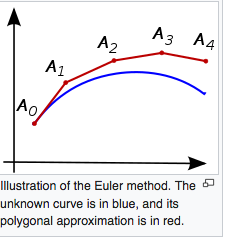
\includegraphics[width=0.49\textwidth]{euler_wikipedia.png}
% % &
% % 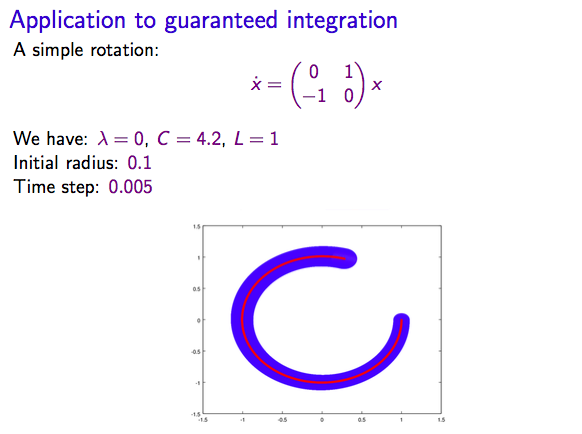
\includegraphics[width=0.49\textwidth]{rotation_Euler.png}
% %\\
% %(a) & (b)
% %\end{tabular}
% %
% % \caption{Illustration of Euler's method.}
% % \label{fig:euler}
% %\end{figure}
% 
% \subsection{Comparison with error bounds based only on Lipschitz constants}
% ---------------
% 
% As said in \cite{NL_minimator}, in the methods of symbolic analysis
% and control of hybrid systems, the way of representing sets of state
% values and computing reachable sets for systems defined by ordinary
% differential equations (ODEs) is fundamental (see, \textit{e.g.},
% \cite{Althoff2013a,girard2005reachability}).  An interesting approach
% appeared recently, based on the propagation of reachable sets using
% guaranteed Runge-Kutta methods with adaptive step size control (see
% \cite{BMC12,immler2015verified}). In \cite{NL_minimator} such
% guaranteed integration methods are used in the framework of {\em
%   sampled switched systems}.
% 
% \todo[inline]{Reprendre l'introduction}
% 
% In contrast, in [SNR17], we use ordinary arithmetic (instead of affine
% arithmetic) and a basic Euler scheme (instead of Runge-Kutta
% schemes). We need neither estimate Lagrange remainders nor perform
% Picard iteration in combination with Taylor models.  This simple
% Euler-based approach is made possible by having recourse to the notion
% of {\em one-sided Lipschitz} (OSL) function \cite{Donchev98}.  This
% allows us to bound directly the {\em global error}, \textit{i.e.}, the distance
% between the approximate point~$\tilde{x}(t)$ computed by the Euler
% scheme and the exact solution $x(t)$ for all $t\geq 0$ (see
% Theorem~\ref{th:1_part4}). Such an evaluation of the error then allows us to
% synthesize a control of hybrid systems (and, more precisely, of
% sampled switched systems) in order to guarantee the satisfaction of
% safety properties.
% \\
% 
% \todo[inline]{Mettre en avant la contribution sur l'efficacite et une
%   alternative aux methodes sensibles au wrapping effect}
% 
% In this paper, we explain how this Euler-based approach can be simply
% extended to treat {\em distributed systems} where each component has
% only partial information on the state of the other components. This
% distributed (or compositional) computation of the error also allows us
% to fight the ``curse of dimensionality'' which happens in treating
% these systems in a centralized manner.
% 
% \section{Related Work}
% \label{sec:relat-work}
% 
% ------------------------
% 
% % }
% % \section{Guaranteed integration methods {\color{red} [Alexandre, Julien]}}
% 
% % 51 ans d'integration validee
% 
% %  1) pb general et initial cond = set, 2) calcul erreur et propagation et wrapping effect
% 
% 
% % \begin{itemize}
% %  \item Moore (formule Taylor + forme centree)
% %  \item Bertz Makino (Lagrange remainder / taylor series)
% %  I: enclosure II: Tightening
% 
% %  Comparaison avec Butcher
% 
% %  \item Lohner
% %  \item Nedialkov
% 
% %  Dynibex
% %  \item Chen, Abraham, Sriram
% 
% %  K\"uhn zonotopes
% 
% %  Girard, Althoff
% 
% %  \item affine arithm. (Goubault, Putot) ``bloating''
% 
% %  \item {\color{green} Jaulin ?}
% % \end{itemize}
% 
% % ------
% % utilisation originale dans ce contexte de la one-sided-Lipschitz (OSL) constant, ``inventee''
% % pour traiter stiff equations + garantir stabilite
% 
% % Related work
% % \begin{itemize}
% %  \item Donze, Maler
% %  \item Kurzanski
% %  \item ellipsoids
% %  \item sensitivity analysis
% %  \item {\color{green}  Thao Dang et complex zonotope templates $\sim$ ellipsoids}
% % \end{itemize}
% 
% % OSL constant $<0$  $\sim$ incremental stability, lyapunov function = norme 2
% 
% 
% % Taylor vs OSL, interet compar\'e, global vs local
% 
% % application: contraction localement avec L.op. {\color{red} (L.op. ???)}\\
% 
% 
% % New method for fighting wrapping effect:
% 
% % - point (instead of polygon): avoids increasing surface/volume due to
% % computation of vertices (ex: rotation)
% 
% % - computation of global error (instead of LTE): avoids accumulation of errors
% % (size step of integration can be bigger - no need of sub-sampling); ex: ???\\
